\chapter{Framework for Efficient Manipulation Task Planning}
\label{chap:proposal-framework}

\begin{figure*}
   \begin{center}
   
   \subfloat[Start config]{%
      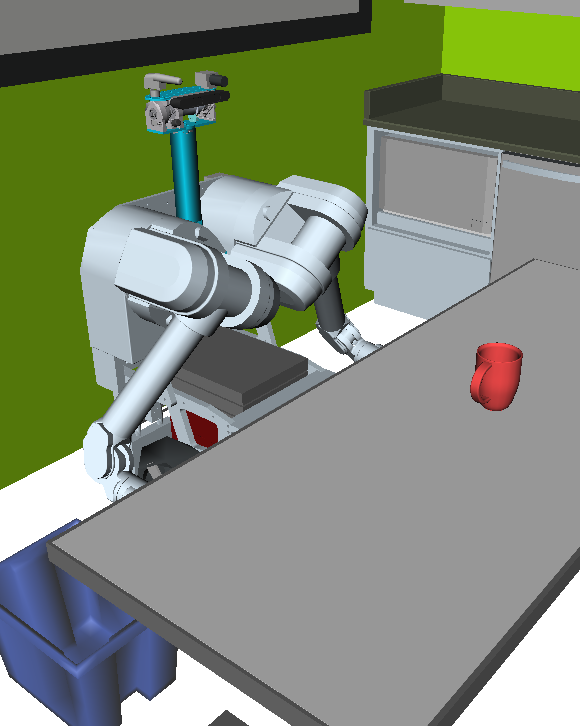
\includegraphics[width=0.19\linewidth]{figs/testherb-a.png}%
   }
   \,
   \subfloat[Step 1 in $X_1$]{%
      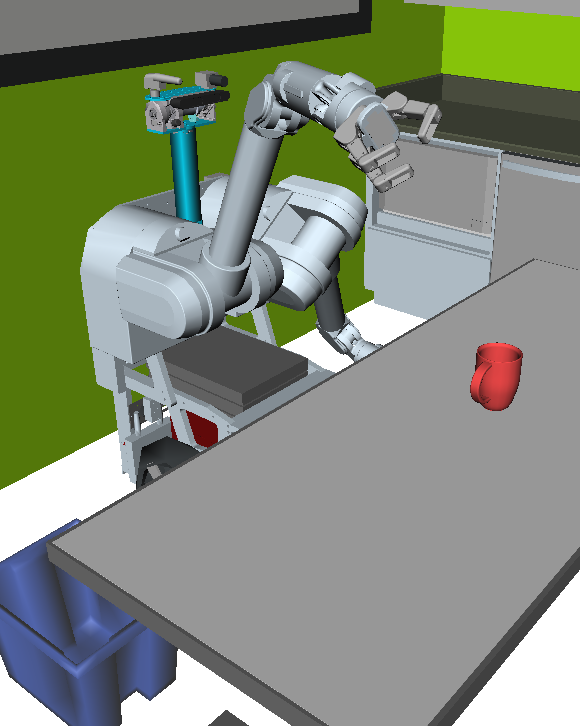
\includegraphics[width=0.19\linewidth]{figs/testherb-b.png}%
   }
   \,
   \subfloat[Step 2 in $X_2$]{%
      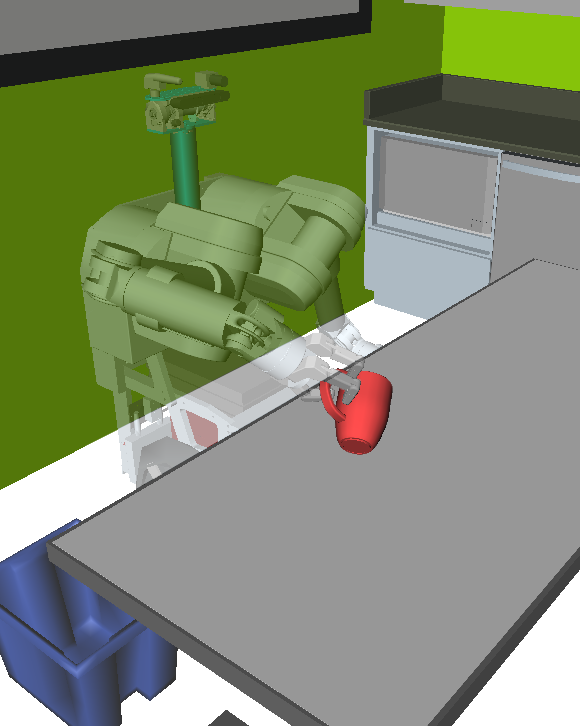
\includegraphics[width=0.19\linewidth]{figs/testherb-c.png}%
   }
   \,
   \subfloat[Step 3 in $X_3$]{%
      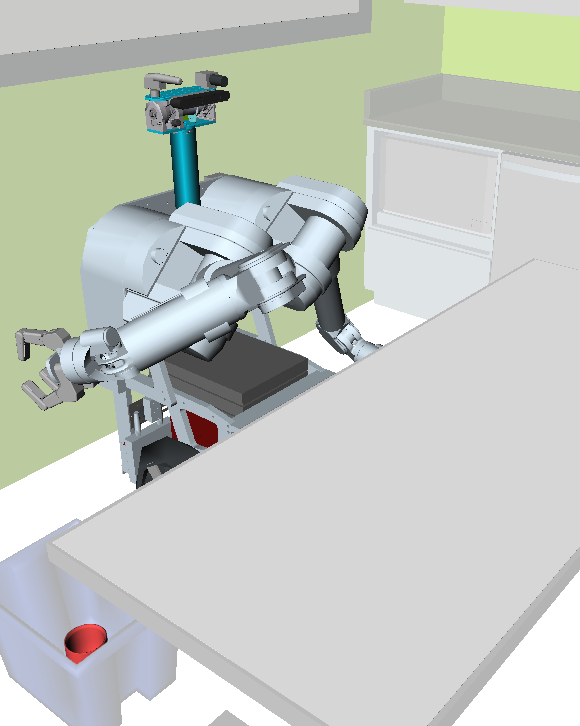
\includegraphics[width=0.19\linewidth]{figs/testherb-d.png}%
   }
   \,
   \subfloat[End config]{%
      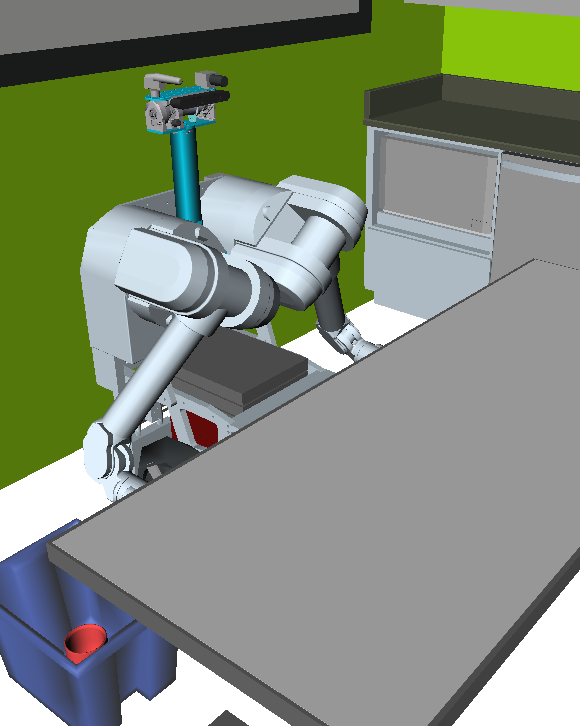
\includegraphics[width=0.19\linewidth]{figs/testherb-e.png}%
   }
   
   \subfloat{
      \includegraphics{build/diagram-multi-step}
   }

   %\caption[][0.2in]{
   %   Diagram of multi-step planning framework.
   %   This thesis focuses on efficient geometric planning
   %   for manipulation tasks (the lower two levels here).
   %   Task planning can be performed by an autonomous
   %   symbolic planner,
   %   or guided by a human operator.}

   \end{center}
   
   \refstepcounter{figure}
   \smallskip\noindent\small Figure \thefigure:
      Diagram of multi-step planning framework.
      This thesis focuses on efficient geometric planning
      for manipulation tasks (the lower two levels here).
      Task planning can be performed by an autonomous
      symbolic planner,
      or guided by a human operator.
   
   \label{fig:xx-diagram-multi-step}
   
\end{figure*}

This chapter lays out our proposed approach
to planning for coupled manipulation tasks.
The reader is directed to
%Figure~\ref{fig:xx-diagram-multi-step}
Figure~2.1
for an overview.
Our approach consists generally of decomposing the task into
multiple steps,
each of which is solved by queries to an underlying motion
planner in the robot's
\emph{configuration space}\cite{lozanoperez1983cspace}.

% from sidd:
%Where to steps come from?
%what do i mean by steps?
%what is a step?
%walking, parkour
%cosntrained door opening
%reaching into a box
%replacing the car tire
%we focus on manipuation
%opening a door are manipuation
%two things that produce structure:
%- cobs
%- cspace manifolds
%we're just looking at a projection of the composite c-space

We suggest that a reasonable decomposition of a task into steps
should be guided by changes to either
the valid subset of the robot's configuration space
(e.g. at grasp and release points of manipulated objects)
or the set of constraints active on the robot's configuration.
This facilitates simpler calls to each motion planner,
and also allows separate planners with different capabilities
(e.g. constrained planners)
to be used for each step.

\textbf{Outline.}
Loosely, the sections in this chapter are layed out as follows.
Sections~\ref{chap:e8} and~\ref{chap:graphs-in-continuous}
describe our approach to planning \emph{within} each step,
on graphs and roadmaps respectively.
Next,
Sections~\ref{chap:multi-set} and~\ref{chap:multi-set-prm}
identify and exploit structure \emph{between} steps
in order to reuse planning computation across queries.
Lastly,
Sections~\ref{chap:cmr} and~\ref{chap:task-planning}
discuss how to specify queries across all steps
in a higher-level sequencing task planner.


\section{Quickly Searching Explicit Expensive Graphs}
\label{chap:e8}

In order for a robot to perform manipulation tasks
in changing, unstructured environments,
it must be able to quickly solve planning queries.
In this section,
we discuss formulating
the motion planning problem as best-first graph search over paths
and propose a search algorithm on explicit graphs.
Our approach is motivated by two insights.

\textbf{Explicit Optimization of Ensemble Effort.}
This section reference two different types of efficiency
with regard to robotic tasks.
First, once a planner has computed a solution path or trajectory,
there is the cost incurred while executing that trajectory.
This is the traditional cost optimized for by planners.
Second, there is the cost incurred from actually computing the solution
itself.
We propose to optimize for both types of effort explicitly.

\textbf{Explicit Graph Representation.}
We contend that representing graphs explicitly
is better suited to search over roadmap graphs
for two reasons.
First, it is reasonable to store the entire graph
\emph{explicitly} in memory
(e.g. ~10k vertices for a 7-DOF arm);
techniques to incrementally build the graph
via an implicit graph representation
are not necessary.
Second,
it is evaluating edge costs
(as opposed to expanding vertices or maintaining
a sorted open list)
that dominates planning costs.
In other words,
precious planning effort is principally manifested in
\emph{evaluated edge costs},
not \emph{determined vertex $g$-values}.

\subsection{Generic Best-First Search Algorithm over Paths}

Best-first search\cite{winston1977ai}
is a general class of search algorithms.
We choose to express the general algorith
over \emph{paths} instead of \emph{vertices}
for clarity and generality
because we are focused primarily on explicit graphs.
%See Algorithm~\ref{alg:generic-best-first}.
\begin{algorithm}
   \caption{Generic Best-First Search Algorithm Outline}
   \label{alg:generic-best-first}
   \begin{algorithmic}[1]
   \Procedure {\textsc{GenericBestFirst}}{$G$}
   \Loop
      \State $\pi^* = \argmin\limits_{\pi \in \Pi} f(\pi)$
         \Comment{For some path cost function $f(\pi)$}
         \label{line:generic-select-optimistic-path}
      \If {$\pi^*$ fully evaluated}
         \State \Return $\pi^*$
      \EndIf
      \State \textsc{EvalPath}$(\pi^*)$
         \Comment{For some evaluation function}
   \EndLoop
   \EndProcedure
   \end{algorithmic}
\end{algorithm}

\noindent
This formulation admits two choices:

\textbf{Cost Function $f(\pi)$.}
What is the cost function $f(\pi)$ over paths used to select the
path for evaluation at each iteration?
For now, we will use the following path objective:
\begin{equation}
   f(\pi) = \hat{f}_x(\pi): \mbox{\emph{optimistic estimate of execution effort}}.
\end{equation}
In other worts, $\hat{f}_x(\pi)$
gives a lower bound on the cost of executing
path $\pi$.
If the path consists of a mix of evaluated and unevaluated edges,
we could write this as:
\begin{equation}
   \hat{f}_x(\pi) = \sum_{e \in \pi} \left\{
   \begin{array}{cl}
      x[e] & \mbox{if edge } e \mbox{ evaluated}  \\
      \hat{x}(e) & \mbox{otherwise} \\
   \end{array}
   \right.
   .
   \label{eqn:execution-cost-objective}
\end{equation}

\textbf{Evaluation Procedure $\mbox{\sc EvalPath}(\pi)$}.
How is a potential path evaluated?

The choice of these two components of the algorithm
intimately depend on the graph representation.
For appropriate selection
of $f(\pi)$ and \textsc{EvalPath},
traditional algorithms such as A* \citep{hart1968astar}
and the Bidirectional Heuristic Front-to-Front Algorithm
\citep{sint1977bhffa}
are instances of this general formulation.

\subsection{Penalizing Planning Effort}

So far, we've been searching for a path which optimizes our execution
effort objective (\ref{eqn:execution-cost-objective}).
However, as we motivated earlier,
there are two distint notions of efficency;
here, we focus instead on \emph{planning efficiency}.
Consider the following path objective:
\begin{equation}
   f(\pi) = \hat{f}_p(\pi) : \mbox{\emph{optimistic estimate of planning effort}}.
\end{equation}

For problems over large graphs,
planning effort may be dominated by discovering vertex successors
or maintaining a sorted vertex open list.
\marginnote{Traditional metrics for evaluating planning
effort include \emph{vertiex expansions}
and \emph{heap percolates}.}.
However, for many manipulation problems,
search time is instead dominated by \emph{edge evaluations}.
Therefore, our objective $\hat{f}_p$
penalizes remaining effort required to evaluate edges
along a potential path:
\begin{equation}
   \hat{f}_p(\pi) = \sum_{e \in \pi} \left\{
   \begin{array}{cl}
      0 & \mbox{if edge } e \mbox{ evaluated}  \\
      \hat{p}(e) & \mbox{otherwise} \\
   \end{array}
   \right.
   .
\end{equation}
The new edge heuristic $\hat{p}(e)$ estimates this evaluation cost.
\marginnote{Suggested metrics for $\hat{p}$
   include planning time or computational energy.}

The first graph planner to explicitly include such a heuristic
to estimate the remaining
computational planning effort in a best-first search
was A$_\epsilon^*$ \citep{pearl1982semiadmissible}.
While the approach we take is different,
a motivating quote from this paper is relevant:
\begin{quote}
``The heuristic [\,$\hat{x}$\,] ... is of an entirely
different nature than the ... heuristic [\,$\hat{p}$\,] ... .
The former anticipates the reduction in \emph{solution quality} due to the
remaining part of the solution once it is found;
the latter estimates the \emph{computational effort}
required for completing the search.''
\end{quote}

\subsection{Ensemble Effort Objective}

In general, we might consider weighting each objective:
\begin{equation}
   f(\pi) = \lambda \hat{f}_p(\pi) + (1 - \lambda) \hat{f}_x(\pi) .
   \label{eqn:general-objective}
\end{equation}
We call this effort model
\emph{ensemble effort}
in that it combines both planning and execution effort.
Note that with $\lambda=0$,
we recover our old solution cost objective $\hat{f}_x(\pi)$.
%Note that this objective is used in an optimistic, greedy fashion at each
%iteration of best-first search.
Represented over edges,
this can then be written:
\begin{equation}
   f(\pi) = \sum_{e \in \pi} \left\{
   \begin{array}{cl}
      (1 - \lambda) x[e] & \mbox{if edge } e \mbox{ evaluated}  \\
      \lambda \hat{p}(e) + (1 - \lambda) \hat{x}(e) & \mbox{otherwise} \\
   \end{array}
   \right.
   .
   \label{eqn:general-objective-explicit}
\end{equation}

We represent a particular choice of $\hat{p}(e)$
and $\hat{x}(e)$,
along with the evaluation function $x(e)$,
as an \emph{ensemble effort model}
denoted with $\mathcal{M}$:
\begin{equation}
   \mathcal{M} : (x, \hat{x}, \hat{p})
\end{equation}

\vspace{0.1in}
\noindent
\textbf{Simplification with Propotional Heuristics}

Suppose that our heuristic for planning effort
were proportional to that for execution effort,
\begin{equation}
   \hat{p}(e) = \alpha \, \hat{x}(e) .
\end{equation}
This might happen if, for example, each were proportional to the edge's
\emph{distance} (with longer paths taking longer to both collision check
and execute at constant velocity).
In this case, we can write:
\begin{equation}
   f(\pi) = (1-\lambda) \sum_{e \in \pi} \left\{
   \begin{array}{cl}
      x[e] & \mbox{if edge } e \mbox{ evaluated}  \\
      \left[ 1 + \frac{\alpha\lambda}{1 - \lambda} \right] \hat{x}(e) & \mbox{otherwise} \\
   \end{array}
   \right.
   .
   \label{eqn:prop-heuristics}
\end{equation}

Consider the case where we're using forward vertex or edge evaluations
(as is required with implicit graph representations),
and $\lambda < 1$.
In this case, we can rewrite (\ref{eqn:prop-heuristics})
simply as:
\begin{equation}
   f(\pi) \propto
   \underbrace{\sum_{e \; \mbox{\scriptsize evaled}} x[e]}_{g[v_f]}
   +
   \underbrace{\left[ 1 + \frac{\alpha \lambda}{1-\lambda} \right]}_{
      \mbox{\scriptsize inflation factor } \epsilon}
   \underbrace{\hat{x}(e_{last})}_{h(v_f)}
   .
\end{equation}

In other words,
\emph{weighted A* is equivalent to
   best-first search whose objective
   includes a planning effort term
   proportional to execution effot.}
In particular, if planning effort is proportional to execution
effort by a factor of $\alpha$,
a weighted A* search with inflation factor $\epsilon$
is the result of best-first search with
$\lambda = \frac{\epsilon-1}{\alpha+\epsilon-1}$.

\subsection{The E$^8$ Explicit Graph Search Algorithm}
\label{sec:e8-planner}

The E$^8$ algorithm
(Exploiting Ensemble Effort Estimates
on Explicit graphs with Expensive Edge Evaluations)
is the result of applying
best-first search with the $\lambda$-mediated objective
from (\ref{eqn:general-objective}).
The algorithm is \emph{lazy},
in that edge evaluations are deferred until they are needed.
In fact, it can be seen as a generalization of the
LazyPRM \citep{bohlin2000lazyprm},
but which also considers planning effort in its objective.
Further,
the algorithm is \emph{heuristic-focused},
guided by its cost model $\mathcal{M}$.
Its behavior mimics that of an inflated heuristic planner
depending on the selection of the planning/execution cost
tradeoff parameter $\lambda$.

\begin{algorithm}[t]
\caption{E$^8$ Explicit Graph Search}
\label{alg:e8}
\begin{algorithmic}[1]
   \Procedure {E$^8$}{$G,
      V_{\mbox{\scriptsize start}}, V_{\mbox{\scriptsize goal}},
      \mathcal{M}, \lambda$}
   \State $x_{\mbox{\scriptsize eval}}[\cdot] \leftarrow$ empty map
      ($x_{\mbox{\scriptsize eval}} : E \rightarrow \mathbb{R}_0^+$)
      \label{line:store-edge-eval-efforts}
   \ForAll {$e \in G$}
      \State $e.{\mbox{cost}} \leftarrow
         \lambda \, \hat{p}(e) + (1 - \lambda) \, \hat{x}(e)$
         \Comment Ensemble effort model $\mathcal{M}$
         \label{line:edge-cost}
   \EndFor
   \Loop
         \label{line:best-first-start}
      \State $\pi^* = \mbox{\sc BiDijkstras}(G,
         V_{\mbox{\scriptsize start}}, V_{\mbox{\scriptsize goal}})$
         \label{line:e8-select-optimistic-path}
      \If {$e \in x_{\mbox{\scriptsize eval}} \;\forall\; e \in \pi^*$}
         \State \Return $\pi^*$
            \label{line:return-done}
      \EndIf
      \State $E_{\mbox{\scriptsize to\_eval}} \leftarrow
         \mbox{\sc PathEvalOrder}(\pi^*)$
         \Comment{See Section \ref{subsec:alg-path-evaluation}}
         \label{line:path-eval-order}
      \ForAll {$e \in E_{\mbox{\scriptsize to\_eval}}$}
         \State $x_{\mbox{\scriptsize eval}}[e] \leftarrow x(e)$
            \Comment Evaluate edge (expensive!)
            \label{line:evaulate-edge}
         \State $e.{\mbox{cost}} \leftarrow
            (1 - \lambda) \, x_{\mbox{\scriptsize eval}}[e]$
            \Comment Update ensemble estimate
            \label{line:update-estimate}
         \If {$x_{\mbox{\scriptsize eval}}[e] > \hat{x}(e)$}
            \label{line:exec-cost-check}
            \State \textbf{break}
               \label{line:eval-break}
         \EndIf
      \EndFor
   \EndLoop
      \label{line:best-first-end}
   \EndProcedure
\end{algorithmic}
\end{algorithm}

The E$^8$ algorithm (Algorithm~\ref{alg:e8})
directly follows the outline
of best-first search over paths
(Algorithm~\ref{alg:generic-best-first}).
Since edge evaluations are expensive,
we maintain a map $x_{\mbox{\scriptsize eval}}[\cdot]$
storing the known execution costs of all edges evaluated so far
(line~\ref{line:store-edge-eval-efforts}).
Each edge's current cost (line~\ref{line:edge-cost})
is derived from the problem's ensemble effort model $\mathcal{M}$.

At each iteration,
we optimistically select the best path $\pi^*$
which minimizes the this ensemble objective.
We select over all paths which connect
a vertex in $V_{\mbox{\scriptsize start}}$
to a vertex in $V_{\mbox{\scriptsize goal}}$
(any-to-any);
for other types of planner specifications,
see Chapter~\ref{chap:cmr}.
We currently implement the algorithm's best-first selection
using a bidirectional variant of
Dijkstra's algorithm \cite{dijkstra1959anote}
on line~\ref{line:e8-select-optimistic-path};
see research question \ref{ques:incremental-search}
for more details.

If this path is already fully evaluated,
we finish on line~\ref{line:return-done}.
Note that if edge costs $x(e)$ may be infinity
(e.g. to denote an infeasible edge),
the algorithm will terminate with a fully evaluated path
with infinite cost if no feasible path exists.

Otherwise,
we evaluate the path's unevaluated edges
(lines \ref{line:path-eval-order}
to \ref{line:eval-break}).
We do this in a particular order,
as discussed later in this section.
For each edge,
we evaluate its execution cost $x(e)$ (line~\ref{line:evaulate-edge})
and update our effort estimate (line~\ref{line:update-estimate})
to account for (a) the actual execution effort
and (b) the fact that no additional planning effort is needed.
If the execution cost of any edge of the path proves
more expensive than we had anticipated
(line~\ref{line:exec-cost-check}),
we break and select a new path.

The E$^8$ algorithm admits a number of choices
which we discuss in the remainder of this section.

\textbf{Choosing $\lambda$.}
The choice of the $\lambda$ parameter
affects the algorithm's tradeoff between planning and execution effort.
See research question \ref{ques:choosing-lambda}
to a discussion about choosing this parameter.

\textbf{Finding the Optimistic-Optimal Path}.
The current implementation of E$^8$ uses
bidirectional Dijkstra's algorithm
(line~\ref{line:e8-select-optimistic-path})
to select the lowest-cost path through the graph
at each iteration of the algorithm.
However, since the cost of only a few edges
are adjusted at each iteration (line~\ref{line:update-estimate}),
it appears to be well-suited to incremental
graph search algorithms (e.g. \cite{koenig2004lpastar}).
See research question \ref{ques:incremental-search}
for discussion regarding improving the efficiency of this search.

\textbf{Selecting the Edge Evaluation Order.}
\label{subsec:alg-path-evaluation}
Once a candidate path is selected,
its constituent unevaluated edges are evaluted
in a particular order (line~\ref{line:path-eval-order}).
Our current algorithm
orders the edges alternating from the ends in.
\cdnote{I need a figure to show this.}
With different choices (e.g. forwards or backwards),
E$^8$ looks a lot like A$^*$.
See research question \ref{ques:evalpath}
for more.

\subsection{Repeated Queries}

The E$^8$ algorithm is \emph{multi-query},
in that it maintains a data structure of evaluated edge
execution costs $x_{\mbox{\scriptsize eval}}[\cdot]$
which allows reuse between different planning problems
over the same graph $G$,
either sequentially or in interleaved fashion.
For different queries on the same graph,
edge evaluations can simply be used in subsequent searches.

When used in this fashion,
E$^8$ behaves similarily to Experience graphs
\cite{phillips2012egraphs}.
E-graphs are a type of best-first search which
are designed to find paths quickly by incentivizing the planner
to rely on on edges from previous successful plans.
While the E-graph planner is originally expressed over implicit graphs,
we can instead express it explicitly
as in Algorithm~\ref{alg:generic-best-first}
with the following objective:
\begin{equation}
   f_{\mbox{\scriptsize E-graphs}}(\pi) \propto \sum_{e \in \pi} \left\{
   \begin{array}{cl}
      x[e] & \mbox{if edge } e \mbox{ evaluated, this search} \\
      \epsilon \, x[e] & \mbox{if edge } e \mbox{ evaluated, previous search} \\
     \epsilon \, \epsilon^E \, \hat{x}(e) & \mbox{otherwise} \\
   \end{array}
   \right.
\end{equation}

The E$^8$ algorithm
is therefore equivalent to a simplified version of the E-Graph algorithm
with $\epsilon=1$ and $\epsilon^E = 1 + \frac{\alpha \lambda}{1-\lambda}$.
with the exception that all evaluated edges are placed in the graph,
not just the edges on the solution path.
Note that E-graph shortcuts
are not necessary for small explicit graphs.

\subsection{Experimental Evaluation of the E$^8$ Algorithm}

We propose to perform experiments on graphs with
expensive edge evaluations
in order to evaluate the E$^8$ algorithm
(see research question \ref{ques:e8-comparisons}).
See Figure~\ref{fig:e8-results} for an example problem.

\begin{figure}[t]
   \centering
   %\begin{center}
   
   % for stats
   \input{build/e8-world-astar-stats}
   \input{build/e8-world-wastar-stats}
   \input{build/e8-world-e8-stats}
   \subfloat[Planning world.]{
      \includegraphics{build/e8-world-intro}
   }
   \quad
   \subfloat[A$^*$ search.
         Planning Effort: 692.3 %\worldstatsastarplan\\
         Execution Effort: 14.2 %\worldstatsastarexec}
   ]{
      \includegraphics{build/e8-world-astar}
   }
   \vspace{0.05in}
   \subfloat[Weighted A$^*$ search, $\epsilon=3$
         Planning Effort: 390.8 %\worldstatswastarplan\\
         Execution Effort: 18.5 %\worldstatswastarexec}
   ]{
      \includegraphics{build/e8-world-wastar}
   }
   \quad
   \subfloat[E$^8$ search, $\lambda=0.5$
         Planning Effort: 358.8 %\worldstatseEplan\\
         Execution Effort: 20.5 %\worldstatseEexec}
   ]{
      \includegraphics{build/e8-world-e8}
   }
   
   \caption{A simple 2D explicit graph search problem,
      comparing three approaches.
      A robot (bottom left) must reach a goal position (top right)
      on an 8-connected graph
      while avoiding a wall (black).
      Execution effort is equal to path length.
      The planning effort required to check an edge is proportional
      to its distance to the blue radar at top.
      The E$^8$ algorithm's solution has a lower combined
      planning and execution effort.}
   \label{fig:e8-results}
\end{figure}

\section{Roadmaps in Continuous Spaces}
\label{chap:graphs-in-continuous}

This section explores how we can construct roadmaps covering
configuration space that can then be searched by the E$^8$ algorithm.
Here,
we focus on the single-query problem;
refer to Section~\ref{chap:multi-set}
for extension to cached data structures.
Due to this focus,
we strive to compare against alternative single-query approaches
as we discuss in Section~\ref{subsec:single-query-results}.

Although
our approach makes no commitment to the roadmap class
(e.g. probabalistic or lattice-based),
we propose to use Random Geometric Graphs (RGGs)
as roadmaps covering configuration space,
borrowing heavily from prior approaches \citep{kavrakietal1996prm}
and analyses \citep{karaman2011samplingoptimal}.
we make no commitment as to the connection strategy
(e.g. $r$-disk or $k$-nearest).
Note that by pre-computing a sequence of samples,
nearest-neighbor queries can be moved entirely offline.
Also,
since it can be computed offline,
you can sparsify it \citep{shaharabani2013sparsification}.

\subsection{The E$^8$-PRM with Hard Batching}

\begin{algorithm}
\caption{E$^8$-PRM Planner with Hard Batching}
\label{alg:e8-prm-hard}
\begin{algorithmic}[1]
\Procedure {E$^8$-PRM}{$
   V_{\mbox{\scriptsize start}}, V_{\mbox{\scriptsize goal}},
   N, \mathcal{M}, \lambda$}
\State $G \leftarrow \mbox{empty graph}$
%\State $G.E \leftarrow \emptyset$
\Loop
   \State \textsc{PrmAddSamples}($G,
      V_{\mbox{\scriptsize start}}, V_{\mbox{\scriptsize goal}},
      N$)
   \State $\pi^* \leftarrow \mbox{E}^8(G,
      V_{\mbox{\scriptsize start}}, V_{\mbox{\scriptsize goal}},
      \mathcal{M}, \lambda)$
      \Comment See Algorithm~\ref{alg:e8}.
   \If {$\hat{x}(\pi^*) < \infty$}
      \Comment $\hat{x}(\cdot)$ from cost model $\mathcal{M}$
      \State \Return $\pi^*$
   \EndIf
\EndLoop
\EndProcedure
\end{algorithmic}
\end{algorithm}

The E$^8$-PRM (Algorithm~\ref{alg:e8-prm-hard})
operates on an initially empty persistent roadmap graph $G$.
Each vertex represents a configuration $q \in \mathcal{C}$,
and each edge represents a path $q(t)$ planned by a local planner.

The E$^8$-PRM proceeds in \emph{batches};
at the start of each batch,
the \textsc{PrmAddSamples} procedure adds
$N$ additional vertices to the graph sampled from $\mathcal{C}$
(including sampled start and goal configurations from
$V_{\mbox{\scriptsize start}}, V_{\mbox{\scriptsize goal}}$
if not yet present),
and edges are generated according to the PRM construction method.

With the exception of the path evaluation strategy
(see Section~\ref{subsec:prm-path-eval}),
the E$^8$-PRM with $\lambda = 0$
is equivalent to 
the Lazy PRM \citep{bohlin2000lazyprm}.

\subsection{Optimization in Expectation}

What graph are we searching over?
If it's too sparse, we'll stop after knowing that no solution exists.
If it's too dense, we'll spend too much time filling in parts of
space.
There's actually some spatial relationship in
$\mathcal{C}_{\mbox{\scriptsize free}}$ that we're not
modeling.
We get around this with artificial sparseness.
There's definitely a paper's worth of work here too (Shushman's stuff).
The easy version is with sequential batches of size $N$.
Talk about how what we really want to do
is evaluate the estimate of cost remaining
\emph{in expectation}.
Relate to Markov Random Fields and two-class image segmentation
which capture spatial correlation.

We propose to extend the E$^8$ search algorithm
to minimize ensemble effort \emph{in expection}
using a probabalistic model of $\mathcal{C}_{\mbox{\scriptsize free}}$.
Even if this is too expensive,
we can motivate the incremental densification idea,
with a graduated cost model
to approximate a probabalistic model
of the $\mathcal{C}$-space.
\marginnote{See research question \ref{ques:batching}.}

\subsection{Path Evaluation}
\label{subsec:prm-path-eval}

In order to use the E$^8$ algorithm,
we must provide an edge evaluation function $x(e)$.
For feasibility checks
(e.g. tested via collision checkers),
we approximate each edge check
by evaluating the corresponding validity checker
at a fixed resolution along the path.

More generally, however,
since the E$^8$-PRM plans in a continuous space,
we can actually implement more complex path tests,
such as the whole-path bisection test used in the
Lazy PRM.
\marginnote{See research question \ref{ques:evalpath}.}

\subsection{Ensemble Effort Models}

The E$^8$ algorithm requires an ensemble effort model
$\mathcal{M}$.
We discuss simple implementations that are useful
for the single-query E$^8$-PRM.
\cdnote{I should talk about how such models can be added.}

\begin{algorithm}
\caption{Validitiy Effort Model
   $\mathcal{M}_{\ms{valid}}$}
\label{alg:single-set-effort-model}
{\algrenewcommand\textproc{}% Used to be \textsc
\begin{algorithmic}[1]
\Function {$x_{\ms{valid}}$}{$e, U$}
   \If {${\bf 1}_U[q_e(t)]$}
      \State \Return $0$
   \Else
      \State \Return $\infty$
   \EndIf
\EndFunction
\Function {$\hat{x}_{\ms{valid}}$}{$e, U$}
   \State \Return $0$
\EndFunction
\Function {$\hat{p}_{\ms{valid}}$}{$e, U$}
   \State \Return $\hat{p}_U[q_e(t)]$
\EndFunction
\end{algorithmic}
} %textproc
\end{algorithm}

\textbf{Planning Cost Models.}
This is the planner in continuous spaces,
requires a planning cost model for each edge.
For single-query planners,
we typically implement $\hat{p}(e)$ to be
proportional to the number of collision checks required
to validate the edge.
See Algorithm~\ref{alg:single-set-effort-model}.

\begin{margintable}
   \centering
   \begin{tabular}{lc}
      \toprule
      Model & Additive? \\
      \midrule
      Path Length & Yes \\
      Bounded-Vel-Acc & Yes \\
      Smoothed & No \\
      \bottomrule
   \end{tabular}
   \vspace{0.1in}
   \caption{Execution cost models.
      Additive models admit efficient graph search methods
      when choosing optimistic paths for evaluation.}
   \label{table:exec-cost-models}
\end{margintable}

\textbf{Execution Cost Models.}
Due to the graph problem representation,
E$^8$ requires additive effort models.
Could we relax the additive execution cost constraint?
We lose the nice efficient LPA*-enabling structure in
E$^8$ this way,
but it lets us incorporate a more accurate cost model in some domains,
especially for execution costs for fast motions (e.g. total time).
See Table~\ref{table:exec-cost-models} for examples.
Sidd wants me to play with Hauser's fast bounded-velocity,
bounded-acceleration segment timing code
(which starts and stops at each waypoint).
This may have better performance,
choosing longer paths with few long edges over
shorter paths with many short edges.

\subsection{Experimental Evaluation of the E$^8$-PRM}
\label{subsec:single-query-results}

\begin{figure}
   \centering
   \subfloat[RRT Ext-Con, R=1]{
      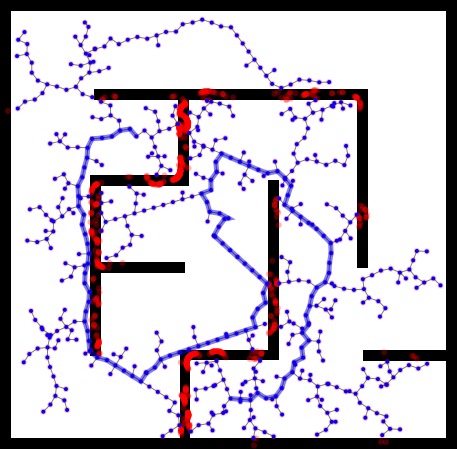
\includegraphics[width=0.3\textwidth]{figs/compare-2d-rrtc1-rrtextcon-r1-s1.png}
   }
   \,
   \subfloat[RRT Con-Con, R=1]{
      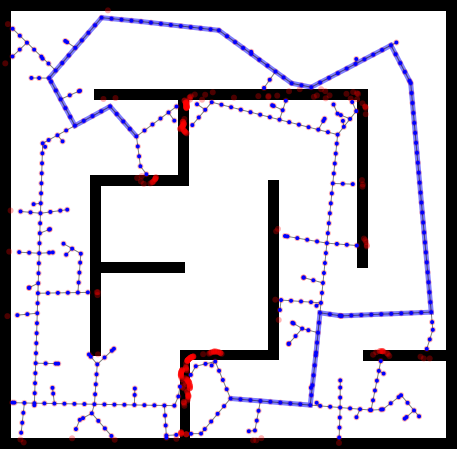
\includegraphics[width=0.3\textwidth]{figs/compare-2d-rrtc1-rrtconcon-r1-s1.png}
   }
   \,
   \subfloat[E$^8$-PRM, $\lambda=0$]{
      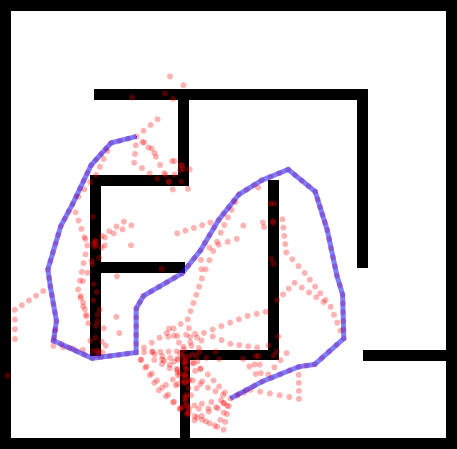
\includegraphics[width=0.3\textwidth]{figs/compare-2d-rrtc1-checkmask-l00-s1.png}
   }
   
   \vspace{0.05in}
   
   \subfloat[RRT Ext-Con, R=6]{
      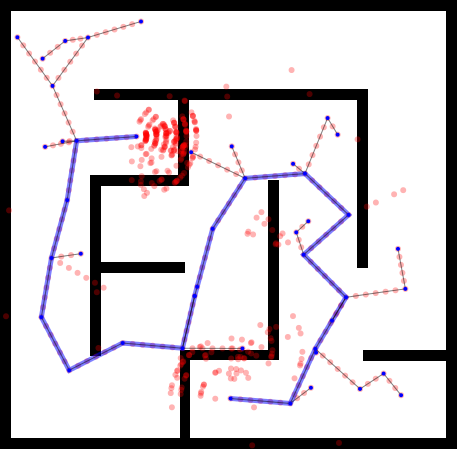
\includegraphics[width=0.3\textwidth]{figs/compare-2d-rrtc1-rrtextcon-r6-s1.png}
   }
   \,
   \subfloat[RRT Con-Con, R=6]{
      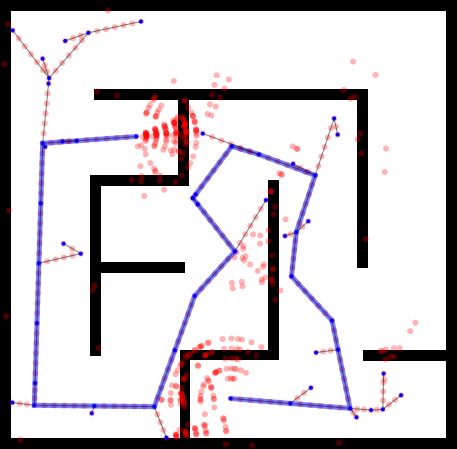
\includegraphics[width=0.3\textwidth]{figs/compare-2d-rrtc1-rrtconcon-r6-s1.png}
   }
   \,
   \subfloat[E$^8$-PRM, $\lambda=1$]{
      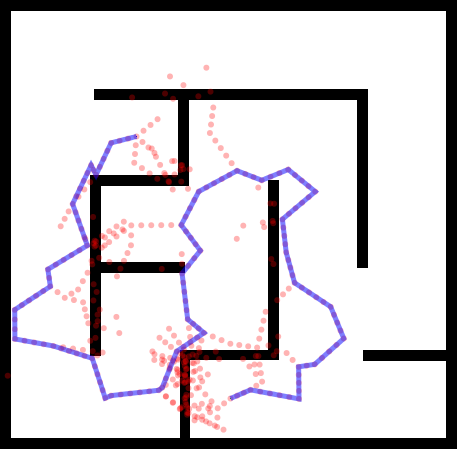
\includegraphics[width=0.3\textwidth]{figs/compare-2d-rrtc1-checkmask-l10-s1.png}
   }
   
   \vspace{0.05in}
   
   \subfloat[Plot of collision checks vs solution path cost for the
         different algorithms.]{
      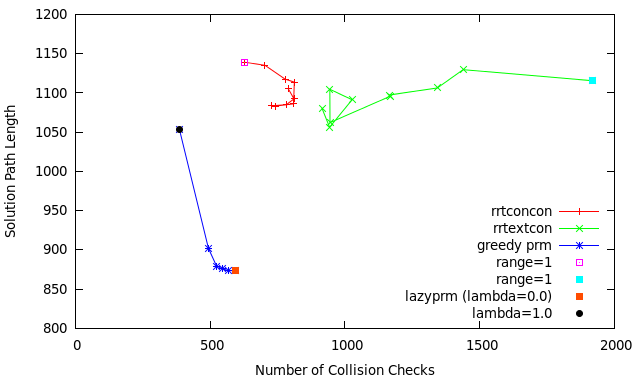
\includegraphics[width=0.8\textwidth]{figs/compare-2d-rrtc1-medians.png}
   }
   
   \caption{Example runs with different planners,
      with the same sequence of samples.
      Note that E$^8$-PRM with $\lambda=0$ is equivalent to the Lazy PRM.
      Red dots show collision checks.}
   \label{fig:compare-2d-rrtc1-vis}
\end{figure}

\begin{figure}
   \centering
   \subfloat[Paths with $\lambda = 0$]{
      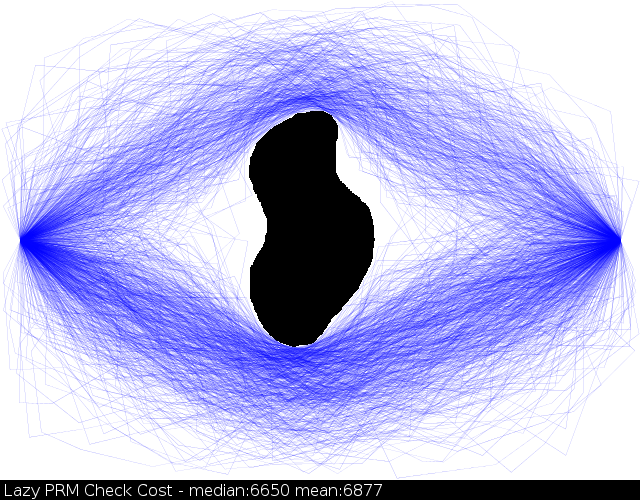
\includegraphics[width=0.45\textwidth]{figs/timegreedy-bean-lambda-00.png}
   }
   \,
   \subfloat[Paths with $\lambda = 1$]{
      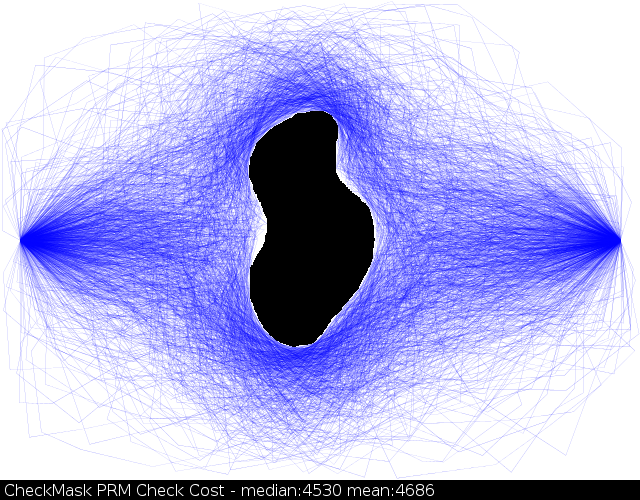
\includegraphics[width=0.45\textwidth]{figs/timegreedy-bean-lambda-10.png}
   }
   \caption{Examples of paths for a 2d problems
      for different values of $\lambda$.
      As $\lambda$ is increased,
      paths are longer, but are faster to find.}
   \label{fig:bean}
\end{figure}

\begin{figure}
   \centering
   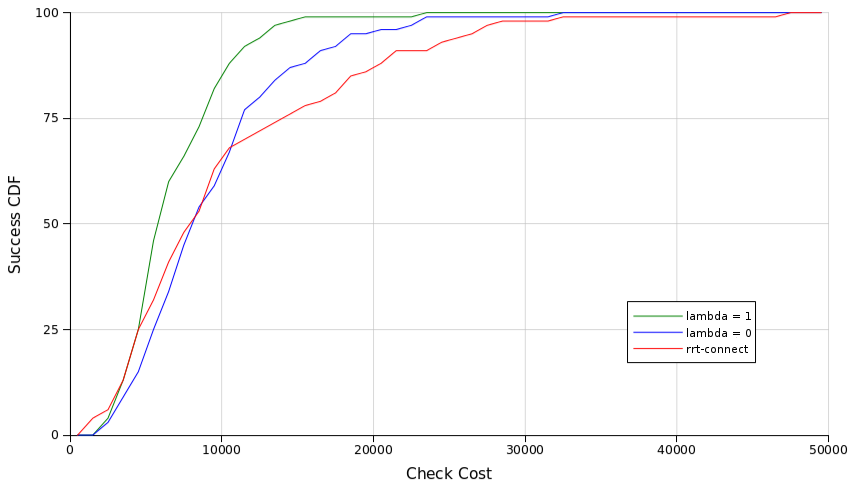
\includegraphics[width=0.8\textwidth]{figs/timegreedy-herbstep1-comparison-cdfs.png}
   \caption{Comparison between different algorithms on a HERB problem.}
   \label{fig:herb-comparison-cdfs}
\end{figure}

I hope to show that the E$^8$-PRM is competitive with RRT-Connect
in terms of planning effort required to find a feasible path.

We will compare this approach to
single-query baseline approaches
such as the RRT \citep{kuffner2000rrtconnect},
EST, SBL \citep{sanchezante2001sbl},
and Lazy PRM \citep{bohlin2000lazyprm},
approaches over lattices such as E-graphs,
as well as asymptotically-optimal planners such as
RRT* \citep{karaman2011samplingoptimal}
and BIT* \citep{gammell2015bitstar}.
Also compare briefly against trajectory optimization approaches,
though these are largely complementary.
For example, there's CHOMP \citep{zucker2013chomp}
and TrajOpt \citep{schulman2013trajopt}.
Defer discussion of caching to subsequent
sections.

See Figures~\ref{fig:compare-2d-rrtc1-vis},
\ref{fig:bean}, and \ref{fig:herb-comparison-cdfs}
for results from some preliminary experiments.

\section{The Multi-Set Planning Problem}
\label{chap:multi-set}

Motion planning approaches that build graphs
in the collision-free subset of
configuration space,
e.g. the
PRM \citep{kavrakietal1996prm}
and RRT \citep{lavallekuffner1999rrt},
have proven promising
for high-dimensional articulated robotics problems
in unstructured environments.
These approaches devote a large amount of computational effort
testing configurations and paths for collision,
and the resulting graph can then be reused
for other queries in the same collision-free subset.
The E$^8$-PRM,
introduced above in Section~\ref{chap:graphs-in-continuous},
is another such approach.

However,
for manipuation problems,
this subset of the robot's configuration space
is sensitive to the locations and shapes of
both people and objects in the environment,
as well as the robot itself.
In addition, it depends on the shape and pose of any object
grasped by the robot.
This makes it difficult not only to apply the results of prior
planning computation to the current problem,
but also to efficiently consider planned or hypothesized motions,
since we must reconstruct our graph from scratch whenever
the environment changes.
This is especially the case for
multi-step manipulation tasks that must be planned into the future.
%We want to continuously update our representation for detours.

A large body of prior work has focused on methods to
improve planning efficiency on manipulation problems.
We show that many of these approaches are
in fact special instances of a more general structure,
which we formulate as the \emph{multi-set planning problem}.

\subsection{Multi-Set Problem Formulation}
\label{sec:multi-set}

\begin{figure*}
\begin{widepage}
\centering

\subfloat[
   A two-part multi-set problem in $\mathcal{C}$,
   first between $q_1$ and $q_2$ through $X_{12}$,
   then between $q_2$ and $q_3$ through $X_{23}$.
   The two free subsets $X_{12}$ and $X_{23}$ are distinct
   but related.
]{
   \includegraphics{build/figstar-a}
}%
\quad%
\subfloat[
   The free subsets are related via other underlying
   subsets of $\mathcal{C}$, with $X_{12}=A \cap B$
   and $X_{23}=A \cap C$.
   A planner solving the first part (from $q_1$ to $q_2$)
   has found paths in $X_{12}$.
]{
   \includegraphics{build/figstar-b}
   \label{subfig:figstar-intersections}
}%
\quad%
\subfloat[
   Due to the set relations,
   a planner solving the second part
   (from $q_2$ to $q_3$ in $X_{23}$)
   can reuse any segment known to be in $X_{12}$
   by checking only for its membership in $C$.
]{
   \includegraphics{build/figstar-c}
}

\vspace{0.1in}

\subfloat[
   A forklift in a parking lot ($q_1$)
   must retrieve an object ($q_2$)
   and reverse park ($q_3$).
   This two-part problem
   requires plans in distinct collision-free
   $\mathcal{C}$-subsets
   $X_{12}$ and $X_{23}$.
]{
   \begin{tabular}{c}
   \includegraphics{build/example-2d-a} \\
   \includegraphics{build/example-2d-b} \\
   \includegraphics{build/example-2d-c} \\
   \end{tabular}
   \label{subfig:figstar-manip-probdef}
}%
\quad%
\subfloat[
   Sets $X_{12}$ and $X_{23}$ are subsets of
   the configuration space of the robot $\mathcal{C}=\mbox{SE}(2)$,
   and can be represented as intersections
   of underlying subsets $A$, $B$, and $C$
   as in Fig.~\ref{subfig:figstar-intersections}.
]{
   \begin{tabular}{c}
   \includegraphics{build/example-2d-d} \\
   \includegraphics{build/example-2d-e} \\
   \includegraphics{build/example-2d-f} \\
   \end{tabular}
}%
\quad%
\subfloat[
   After planning a path from $q_1$ to $q_2$ (top),
   a planner can reuse a configuration in $X_{12}$ (middle)
   by checking only for its membership in subset $C$,
   resulting in plan reuse (bottom).
]{
   \begin{tabular}{c}
   \includegraphics{build/example-2d-g} \\
   \includegraphics{build/example-2d-h} \\
   \includegraphics{build/example-2d-i} \\
   \end{tabular}
}

\caption[][0.2in]{An illustration of a multi-set planning
  problem in a common configuration space $\mathcal{C}$.
  The problem definition generalizes to an artibrary number of
  configuration space subsets and set relations between them.
  When two queries in different subests are solved sequentially,
  a multi-set planner can reuse path segments less expensively.
  See Section~\ref{sec:in-manipulation} for examples in
  manipulation.}
\label{fig:multi-set}

\end{widepage}
\end{figure*}

Here we define the multi-set planning problem,
a generalization of both the movers' problem
and the multi-query planning problem%
\cite{kavrakietal1996prm}.
The reader is referred to
Fig.~\ref{fig:multi-set}
for a general example,
as well as a simple instantiation in a 2D manipulation task.
%which is discussed in more detail in
%Section~\ref{subsec:multi-prm-example}.
The multi-set problem formulation
explicitly captures both planning and execution effort
and can therefore be used as an ensemble effort model
for use in the E$^8$-PRM planner across queries.

\begin{marginfigure}
   \centering
   \subfloat[Multi-query planning]{
      \includegraphics{build/query-to-subset-a}
   }
   \vspace{-0.05in}
   \subfloat[Multi-set planning]{
      \includegraphics{build/query-to-subset-b}
   }
   \vspace{0.1in}
   \caption{While queries in multi-query planning reference
     the same subset of $\mathcal{C}$,
     each multi-set query references one of a number of such sets.}
   \label{fig:query-to-subset}
\end{marginfigure}

The multi-set planning problem is multi-query in
a fixed configuration space $\mathcal{C}$.
However, unlike related problems in which all
queries demand solution paths contained within a single common subset of
$\mathcal{C}$
(usually the set of collision-free configurations, denoted
$\mathcal{C}_{\mbox{\scriptsize free}}$),
the multi-set problem allows for the specification of
\emph{multiple} such $\mathcal{C}$-subsets
$\mathcal{S} = \{ A, B, \dots \}$.
Like $\mathcal{C}_{\mbox{\scriptsize free}}$,
each member of $\mathcal{S}$
is a subset of the common configuration space
(that is,
$X \subseteq \mathcal{C} \;\forall\; X \in \mathcal{S}$).
For example, in Fig.~\ref{subfig:figstar-manip-spaces},
$\mathcal{C}$-subset $B$
consists of configurations
free of collision between the robot and
the initial object pose.

The problem supports an arbitrary number of queries $\mathcal{U}$.
Each query $u$ references a \emph{single}
$\mathcal{C}$-subset $U \in \mathcal{S}$
(see Fig~\ref{fig:query-to-subset}):
\begin{equation}
  u : ( q_{start},\; q_{goal},\; U ) .
  \label{eqn:q}
\end{equation}
A continuous feasible solution path $q(t)$ must then satisfy
\begin{equation}
  \begin{array}{c}
  q(t) \in U \;\forall\; t \in [0,1] \\
  q(0) = q_{start},\; q(1) = q_{goal} . \\
  \end{array}
  \label{eqn:solution}
\end{equation}
Eqns. (\ref{eqn:q}), (\ref{eqn:solution})
specify single configurations
$q_{start}$ and $q_{goal}$,
but the formulation is trivially extended to start/goal sets.

While simple problems may admit explicit representations of
subsets of $\mathcal{C}$,
recent approaches to complex problems
(e.g. sampling-based planners)
instead reason implicitly via test function(s)
\citep{lavalle2006planningbook}.
To capture this,
we endow each $\mathcal{C}$-subset $X \in \mathcal{S}$ with an
\emph{indicator function} $\mathbf{1}_X(q)$:
\begin{equation}
  \mathbf{1}_X(q) =
    \left\{ \begin{array}{ll}
      \mbox{True} & \mbox{if } q \in X \\
      \mbox{False} & \mbox{otherwise}.
    \end{array} \right.
  \label{eqn:indicator-function}
\end{equation}
Equivalently, the set itself can be defined w.r.t. its indicator:
\begin{equation}
  X = \{ q \in \mathcal{C} \;|\; \mathbf{1}_X(q) = \mbox{True} \} .
\end{equation}

\begin{marginfigure}
   \centering
   \subfloat[Containment relation]{
      \begin{tabular}{cc}
      \includegraphics{build/relations-inclusion} \\
      $A \subseteq B$ \\
      $\mathbf{1}_A \Rightarrow \mathbf{1}_B$ \\
      \end{tabular}
   }
   \vspace{-0.05in}
   \subfloat[Intersection relation]{
      \begin{tabular}{cc}
      \includegraphics{build/relations-intersection} \\
      $A = B \cap C$ \\
      $\mathbf{1}_B \wedge \mathbf{1}_C \Rightarrow \mathbf{1}_A$ \\
      \end{tabular}
   }
   \vspace{0.1in}
   \caption{Types of subset relations.
     Each relation can be expressed directly as set relations
     or equivalently as logical statements
     on the corresponding indicator functions
     $\mathbf{1}_X(\cdot)$.}
   \label{fig:relations}
\end{marginfigure}

Excusing the abuse of notation,
we define an analogous indicator functional $\mathbf{1}_X[\cdot]$
which operates on path segments $q(t)$.
We use parentheses for functions and brackets for functionals.
\begin{equation}
  \mathbf{1}_X[q(t)] =
    \left\{ \begin{array}{ll}
      \mbox{True} & \mbox{if } q(t) \in X \;\forall\; t \in [0,1] \\
      \mbox{False} & \mbox{otherwise}.
    \end{array} \right.
  \label{eqn:indicator-functional}
\end{equation}
Common examples of such indicators
(\ref{eqn:indicator-function}) or (\ref{eqn:indicator-functional})
include validity checkers for
geometric (workspace) collision,
stability, and visibility constraints.
Note that for complex problems,
evaluation of these indicators 
tends to dominate planning effort.

Finally, the multi-set problem incudes a list of set relations
$\mathcal{R}$
between the $\mathcal{C}$-subsets in $\mathcal{S}$.
These can be expressed directly using set theoretic relations,
or equivalently as logical statements
on the corresponding indicator functions.
Common types of such relations
(containment and intersection)
are illustated in Fig.~\ref{fig:relations}.
Fig.~\ref{fig:multi-set} gives an example of intersection relations;
an example of containment is a padded (conservative)
robot model (see Section~\ref{subsec:broad-phase}).

Together, these four elements
(a configuration space $\mathcal{C}$,
subsets $\mathcal{S}$ each with endowed indicators,
a set of queries $\mathcal{U}$,
and a list of subset relations $\mathcal{R}$)
comprise a multi-set planning problem.

\textbf{Example Problem.}
Consider the diagram from Fig.~\ref{fig:multi-set}.
$\mathcal{S}$ consists of five $\mathcal{C}$-subsets labeled
$A$, $B$, $C$, $X_{12}$, and $X_{23}$,
and we have two queries,
$u_{12}: (q_1, q_2, X_{12})$
and
$u_{23}: (q_2, q_3, X_{23})$.
$\mathcal{R}$ consists of the two relations
$X_{12} = A \cap B$ and $X_{23} = A \cap C$.
Suppose a cost model $\mathcal{M}$
wherein evaluating the indicator
$\mathbf{1}_A$ incurs cost 4,
evaluating $\mathbf{1}_B$ and $\mathbf{1}_C$ incurs cost 2,
and evaluating $\mathbf{1}_{X_{12}}$ and $\mathbf{1}_{X_{23}}$
incurs cost 6.
In the manipulation example in
Fig.~\ref{subfig:figstar-manip-probdef},
this would be the case if each
pairwise outlined shape collision check incurs unit cost.

Suppose a graph structure within ${X_{12}}$ has been grown to solve
the first query $u_{12}$.
During the subsequent solve of query $u_{23}$,
an existing path segment known to be in ${X_{12}}$ can be shown to
also be contained within ${X_{23}}$ by only evaluating $\mathbf{1}_C$.
In the manipulation example,
reusing an a configuration from the previous search
would require only a check of cost 2,
instead of cost 6 for a new configuration.
Thus, we might hope that a planner may be biased towards reusing
said path segments in this case.

\subsection{Multi-Set Problems in Manipulation Tasks}
\label{sec:in-manipulation}

Instances of multi-set problems are especially prevalent when
planning for manipulation tasks with articulated robots.
This section details several such instances.
While these instances are discussed separately here,
they are often present simultaneously.
See Section~\ref{subsec:herb-experiment}
for experimental results for a problem
which includes several of the multi-set problem instances
described below.

We also provide an implementation for the
OpenRAVE \citep{diankov2010openrave}
virtual kinematic planning environment
which automatically discovers $\mathcal{C}$-subsets
in manipulation tasks.

\vspace{0.1in}
\noindent
\textbf{Dynamic Environments}
\label{subsec:dynamic-environments}

\begin{figure}
   \centering

   \begin{minipage}{.6\textwidth}
      \begin{tikzpicture}
      \tikzset{>=latex} % arrow heads
      \node[anchor=south west,inner sep=0] at (0,0)
        {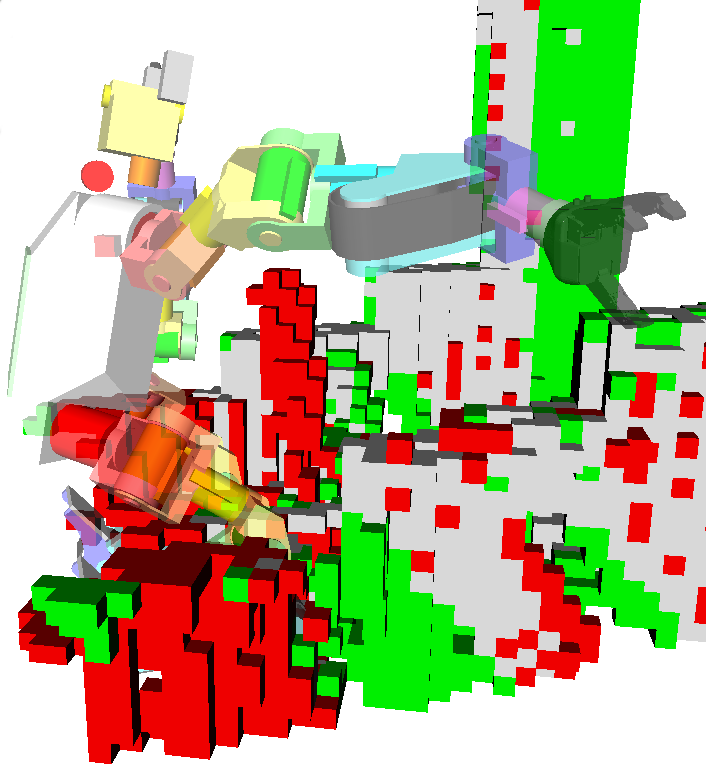
\includegraphics[width=0.8\textwidth]{figs/chimp-voxels-delta.png}};

      \node[draw,inner sep=3pt,fill=white,fill opacity=0.9,align=center]
        (debrislab) at (0.7,1.0) {Debris object\\removed};
      \node[circle,inner sep=2,draw,fill=white] (debris) at (2.2,2.9) {};
      \draw[draw=black, double=white, double distance=1pt, line width=1pt]
        (debrislab.north) -- (debris);
        
      \node[draw,inner sep=3pt,fill=white,fill opacity=0.9,align=center]
        (addlab) at (5.0,2.0) {Additional\\voxels seen};
      \node[circle,inner sep=2,draw,fill=white] (added) at (4.4,5.0) {};
      \draw[draw=black, double=white, double distance=1pt, line width=1pt]
        (addlab.north) -- (added);
        
      \end{tikzpicture}
   \end{minipage}%
   \,%
   \begin{minipage}{.35 \textwidth}
      \includegraphics{build/retroactive-a}
      
      \includegraphics{build/retroactive-b}
   \end{minipage}

   \caption{
      Structured or unstructured dynamic environments
      can be represented as a multi-set problem
      (see Section~\ref{subsec:dynamic-environments}).
      
      \vspace{0.05in}
      \noindent
      (Left) A disaster response robot maintains a
      dynamic unstructured environment model
      using coarse voxels
      (scene data from a debris-clearing task at a
      recent disaster response competition).
      Since the last planning query,
      voxels have been added (green) and removed (red).
      
      \vspace{0.05in}
      \noindent
      (Right) $\mathcal{C}$-subsets and relations
      can be added retroactively.
      Here, the graph for an initial query is checked w.r.t $X_1$.
      After environment changes,
      $X_1$ is redefined in terms of the $\mathcal{C}$-subsets
      derived from the set of common, added, and removed elements,
      allowing for reuse on a query in $X_2$.
      Here,
      the planner need only check existing path segments
      against added voxels in order to reuse them for the current query.}
   \label{fig:dynamic-environments}
   %\label{fig:retroactive}
\end{figure}

The sensors on most articulated robots allow them to maintain
dynamic environment models to track changing collision geometry
(see Fig.~\ref{fig:chimp-voxels-delta}).
These models might be
structured (e.g. recognizing objects with known models)
or unstructured (e.g. occupancy models).
In both cases,
even in a changing world,
there are often areas that are fixed between planning queries.

Prior work (e.g. \citep{jaillet2004dynamicprm})
leverages this by imposing a dichotomy between
\emph{fixed} and \emph{moving} components of $\mathcal{C}$.
Our formulation extends this to an arbitrary number of such labels,
including ones defined retroactively (i.e. during planning;
see Fig.~\ref{fig:retroactive}).
By explicitly labeling such areas in workspace
(and leveraging the \emph{set containment} property
\citep{newmanbranicky1991cspacetransforms}),
we can represent this structure as a multi-set planning problem.

Special case of this is if objects are disappearing.

Relation to occupancy grid representations of workspace
(for deltas, conservative approxs, etc).

\vspace{0.1in}
\noindent
\textbf{Grasped Objects}
\label{subsec:grasped-objects}

One instance specific to manipulation problems is the handling of
grasped objects.
For example, 
consider a manipulator which grasps a geometric object.
This affects the set of collision-free configurations
across a large section of $\mathcal{C}$
relative to the old set of valid configurations $X_{old}$.
However,
the resulting $\mathcal{C}$-subset $X_{new}$
can be represented simply as
$X_{new} = X_{old} \cap G$,
with $G$ the set of robot configurations in which
the \emph{grasped object} (only)
is deemed free of collision with the robot and environment.
This structure is discussed in the context of the
\emph{conditional reachability graph},
part of the \textsc{FFRob} heuristic framework
\citep{garrett2014ffrob}.

For example,
consider the manipulation problem in
Figure~\ref{fig:testherb-problem}.
The robot must find a path which moves its arm to grasp the cup.
After the cup is grasped,
the robot can reuse any edge in the existing roadmap
by simply checking the grasped cup
against the remainder of the environment.
This structure,
together with the approach to dynamic environments,
are included together in the experimental results
(Section~\ref{subsec:herb-experiment}).

\begin{marginfigure}
   \centering
   \includegraphics{build/self-collision}
   \caption{A roadmap is pre-computed in $R$,
      the subset of $\mathcal{C}$ consisting of configurations free
      of robot self-collision.
      Online, the planner must find a path that's also within $E$,
      the subset free of environment collision.
      When solving this query in $X = R \cap E$,
      the Multi-Set PRM automatically prefers potential paths with
      pre-computed edges (e.g. shown in grey)
      due to lower planning costs over alternatives with lower
      execution costs.}
   \label{fig:self-collision-example}
\end{marginfigure}

\vspace{0.1in}
\noindent
\textbf{Cached Self-Collision-Checked Roadmaps}
\label{subsec:cached-self-valid}

Self-collision checking is a potentially expensive component to
articulated motion planning;
in contrast to environment checking,
it is fundamentally quadratic in the number of moving links.
Further, pairs of links to be checked
tend to be relatively close to each other,
reducing the effeciveness of broad-phase approaches.

Leven and Hutchinson \citep{leven2000changing}
introduced the concept of a pre-cached roadmap consisting of
configurations and paths already known to be valid w.r.t.
self-collision.
As a type of invariant in $\mathcal{C}$,
this can be seen as a particular instance of multi-set planning.
See Fig.~\ref{fig:self-collision-example}.

\begin{figure*}[t]
   \centering
   
   \subfloat[
      A single-set planner testing simply for membership in
      $\mathcal{C}_{\mbox{\scriptsize free}}$
      treats a collision validity checker as a
      ``black box.''
      Internally,
      modern checkers first employ an inexpensive broad-phase check
      using a low-dimensional conservative representation
      to quickly identify non-colliding bodies before
      resorting to an expensive narrow-phase check.
   ]{
      \includegraphics{build/broadphase-single}
   }%
   \quad%
   \subfloat[
      A multi-set planner can explicitly reason about the
      conservative nature of the broad-phase check.
      This allows it to defer some narrow phase checks
      (often indefinitely)
      and instead prefer paths that require fewer expensive checks.
   ]{
      \includegraphics{build/broadphase-multi}
   }
   
   \caption[][0.2in]{Collision validity checking is a commonly used
     indicator function.
     The multi-set formulation allows an intelligent planner to
     reach inside the checker's ``black box'' and reduce the number
     of costly narrow-phase checks.
     Resulting paths tend to be cheaper to compute and
     stay further from obstacles.}
   \label{fig:broad-phase}
\end{figure*}

\vspace{0.1in}
\noindent
\textbf{Integration with Broad-Phase Collision Checking}
\label{subsec:broad-phase}

The multi-set formulation also enables motion planners to
reason directly about different robot or environment models.
For example, consider two geometric robot models,
one with high quality (e.g. from a CAD program),
and one hand-tuned ``padded'' model consisting of 
a small number of simple conservative bounding volumes.
The $\mathcal{C}$-subsets derived from these models
are related by $R_{padded} \subseteq R_{CAD}$.
Collision checkers currently use a similar approach internally
to speed up collision checks (see Fig.~\ref{fig:broad-phase}.
and Fig~\ref{fig:broad-phase-2d}).

%\subsubsection*{Conservative Bounding Volumes for Different Grasps}
%
%\subsubsection*{Conservative Bounding Volumes for Hypothesized Objects}
%
%There's a sweet ICRA paper here.
%
%\subsubsection*{Dual Arm Stuff}
%
%I think this is related.
%
%Check right arm against gian left side box, etc.
%
%\subsubsection*{Dimensionality Reduction}
%
%The Handey \cite{lozanoperez1987handey} robot
%assumed a box that contained the wrist links at a range of DOF values.
%
%\subsubsection*{Dual-Arm Stuff}
%
%This is very similar to dimensionality reduction.
%
%Loose coupling between arms.
%
%Separate roadmaps for each arm.
%
%Investigate this multi-set structure.




\section{Multi-Set as a Planning Cost Model for Roadmap Planners}
\label{chap:multi-set-prm}

Our second key insight
is to apply the principle of best-first search over roadmaps
using an objective which explicitly considers both planning and
execution costs.
The result is the Multi-Set PRM.
This approach allows the planner to exploit the multi-set structure
inherent in these problems.

\subsection{The Multi-Set PRM}

\cdnote{I must explain how this works here.}

\begin{algorithm}
\caption{Multi-Set PRM Planner with Hard Batching}
\label{alg:multi-set-prm-hard}
\begin{algorithmic}[1]
\Procedure {MultiSetPRM}{$G,
   V_{\ms{start}}, V_{\ms{goal}},
   N, \lambda$}
%\State $G \leftarrow \mbox{empty graph}$
\State $P_{\ms{global}} \leftarrow
   \mbox{global propositions from\;} \mathcal{R}$
%\State $\mathcal{M} \leftarrow
%   \left\{ \, {\hat p}_{Xu}(\cdot), \, {\hat x}(\cdot) \, \right\}$
\Loop
   \State \textsc{PrmAddSamples}($G,
      V_{\ms{start}}, V_{\ms{goal}},
      N$)
   \State $\pi^* \leftarrow \mbox{E}^8(G,
      V_{\ms{start}}, V_{\ms{goal}},
      \mathcal{M}, \lambda)$
      \Comment See Algorithm~\ref{alg:e8}.
   \If {$\hat{x}(\pi^*) < \infty$}
      \Comment $\hat{x}(\cdot)$ from cost model $\mathcal{M}$
      \State \Return $\pi^*$
   \EndIf
\EndLoop
\EndProcedure
\end{algorithmic}
\end{algorithm}

\subsection{An Ensemble Effort Model for Multi-Set Problems}
\label{subsec:cost-model}

While the indicators
(\ref{eqn:indicator-function}) and (\ref{eqn:indicator-functional})
are binary,
we are often interested not only in solution feasibility,
but also minimizing a measure of \emph{execution cost}
on the solution path.
Furthermore,
\emph{planning cost} is often also an important consideration.
Here,
we define a cost model $\mathcal{M}$
for multi-set problems
which allows these costs to be captured.

%\subsubsection*{Execution Cost}
We capture the expected execution cost of a candidate path
$q(t)$ in the space of $\mathcal{C}$-space paths $H$
via a simple functional ${\hat x}[\cdot]$:
\begin{equation}
  \hat{x} : H \rightarrow \mathbb{R}_0^+ .
\end{equation}
We assume that $\hat{x}[q(t)]$ is known and inexpensive to compute.
Common metrics include
execution time (s) or energy (J).

%\subsubsection*{Planning Cost}
Since indicator evaluation tends to dominate planning costs
in sampling-based planners,
we choose to explicitly penalize such evaluations.
In particular,
each call to indicator functional $\mathbf{1}_X[\cdot]$
incurs a cost given by ${\hat p}_X[\cdot]$:
\begin{equation}
  {\hat p}_X : H \rightarrow \mathbb{R}_0^+ .
\end{equation}
We assume that ${\hat p}_X[\cdot]$ itself is inexpensive to compute.
Common estimates include expected collision checking time (s)
or computational energy required (J).
Often, ${\hat p}_X[q(t)]$ is proportional to both
the length of the path $q(t)$
and a fixed estimate of the complexity of $\mathcal{C}$-subset $X$.

Together, the execution cost functional ${\hat x}[\cdot]$
and the planning cost functionals
${\hat p}_X[\cdot] \;\forall\; X \in \mathcal{S}$
comprise the multi-set ensemble effort model $\mathcal{M}$.
Note that representing all functionals in common units
(e.g. seconds or Joules) allows a planner
to effectively trade off between planning and execution cost.

\begin{algorithm}
\caption{Multi-Set Validitiy Effort Model
   $\mathcal{M}_{\ms{multi}}$}
{\algrenewcommand\textproc{}% Used to be \textsc
\begin{algorithmic}[1]
\Function {$x_{\ms{multi}}$}{$e, U$}
   \State $({\hat p}_{\ms{cert}}, \mathcal{S}_{\ms{cert}}, b_{\ms{cert}})
      \leftarrow \mbox{\sc MultiOptCert}(q_e, U,
      P_{\ms{global}} \cup e.P_{\ms{eval}})$
   \ForAll {$X \in \mathcal{S}_{\ms{cert}}$}
      \State $b_{\ms{eval}} \leftarrow \mathbf{1}_X[q_e]$
      \State $\arraycolsep=2pt
         e.P_{\ms{eval}} \leftarrow e.P_{\ms{eval}} \cup
         \left\{\begin{array}{rl}
         \mathbf{1}_X & \mbox{if } b_{\ms{eval}} \\
         \lnot \mathbf{1}_X & \mbox{otherwise} \\
         \end{array}
         \right\}$
      \If {$b_{\ms{eval}} \neq b_{\ms{cert}}(X)$}
         \State \Return $\infty$
      \EndIf
   \EndFor
   \State \Return $0$
\EndFunction
\Function {$\hat{x}_{\ms{multi}}$}{$e, U$}
   \State \Return $0$
\EndFunction
\Function {$\hat{p}_{\ms{multi}}$}{$e, U$}
   \State $({\hat p}_{\ms{cert}}, \mathcal{S}_{\ms{cert}}, b_{\ms{cert}})
      \leftarrow \mbox{\sc MultiOptCert}(q_e, U,
      P_{\ms{global}} \cup e.P_{\ms{eval}})$
   \State \Return ${\hat p}_{\ms{cert}}$
\EndFunction
\end{algorithmic}
} %textproc
\end{algorithm}

\subsection{Calculating the Multi-Set Optimistic Certificate}
\label{subsec:alg-opt-path-cost}

The execution cost component is given by ${\hat x}[q(t)]$
as defined in the cost model $\mathcal{M}$
(Section~\ref{subsec:cost-model}).
The optimistic estimate of the remaining planning cost for the path
is computed by determining the cost of the optimistic plan for each
edge using the \textsc{MultiOptCert} function.

The \textsc{MultiOptCert} function (Alg.~\ref{alg:opt-edge-plan})
performs the core reasoning which exploits the relations in
the multi-set problem.
Before discussing its implementation,
we first briefly discuss the propositional logic approach
used to reason about the state of each edge.

The planner represents the list of set relations $\mathcal{R}$
(Section~\ref{chap:multi-set})
specified in the multi-set problem formulation
as a set of \emph{logical propositions} $P_{rels}$
which are considered globally applicable.
For example,
the proposition $\mathbf{1}_A \Rightarrow \mathbf{1}_B$
follows from the relation $A \subseteq B$
(see Fig.~\ref{fig:relations}).
In addition,
each edge $e$ in the roadmap is augmented with an initially empty
set $e.P$ containing all additional edge-specific propositions
known to be true as a result of any indicator functions evaluated
over that edge.
For example,
if planner evaluated the indicator $\mathbf{1}_B[e]$
and it returned False,
the proposition $\lnot\mathbf{1}_B$ would be added to $e.P$.
Together, such sets of propositions can be used as \emph{premises}
as part of an \emph{argument} to demonstrate a \emph{conclusion};
a logical solver can then be used validate or invalidate the argument.
For example, an argument with these premises and conclusion
$\{ (\mathbf{1}_A \Rightarrow \mathbf{1}_B), (\lnot\mathbf{1}_B) \}
\Rightarrow (\lnot\mathbf{1}_A)$
can be shown to be valid.

\begin{algorithm}
\caption{Multi-Set Optimistic Certification}
\label{alg:opt-edge-plan}
\begin{algorithmic}[1]
\Function {MultiOptCert}{$q_e, U, P_{\ms{known}}$}
   \State $\mathcal{T}_{\ms{imply}} \leftarrow \emptyset$
   \ForAll {$\mathcal{S}_{\ms{cert}} \in \mathcal{P}(\mathcal{S})$}
         \label{line:power-set}
      \State ${\hat p}_{\ms{cert}} \leftarrow \sum_{X \in \mathcal{S}_{\ms{cert}}} \hat{p}_X[q_e]$
      \ForAll {$b_{\ms{res}} \mbox{ \textbf{s.t.} }
            b_{\ms{res}} : \mathcal{S}_{\ms{cert}} \rightarrow \{\mbox{True},\mbox{False}\}$}
            \label{line:all-binary-functions}
         \State $\arraycolsep=2pt
            P_{\ms{res}} \leftarrow
            \left\{\left. \begin{array}{rl}
            \mathbf{1}_X & \mbox{if } b_{\ms{res}}(X) \\
            \lnot \mathbf{1}_X & \mbox{otherwise} \\
            \end{array}
            \right|
            X \in \mathcal{S}_{\ms{cert}}
            \right\}$
         \If {$P_{\ms{known}} \cup P_{\ms{res}}
               \Rightarrow \mathbf{1}_U$ is valid}
            \State $\mathcal{T}_{\ms{imply}} \leftarrow
               \mathcal{T}_{\ms{imply}} \cup
               \{ ({\hat p}_{\ms{cert}}, \mathcal{S}_{\ms{cert}}, b_{\ms{res}}) \}$
         \EndIf
      \EndFor
   \EndFor
   \State \Return $({\hat p}_{\ms{cert}}, \mathcal{S}_{\ms{cert}}, b_{\ms{res}})
      \in \mathcal{T}_{\ms{imply}}$
      with lowest ${\hat p}_{\ms{cert}}$
\EndFunction
\end{algorithmic}
\end{algorithm}

The \textsc{MultiOptCert} function (Alg.~\ref{alg:opt-edge-plan})
is tasked with computing
the optimistically optimal set of indicator evaluations to perform
for the edge in order to validate its membership in the query
$\mathcal{C}$-subset $X_g$.
The function returns three elements:
(a) the set of $\mathcal{C}$-subsets $S \subseteq \mathcal{S}$
whose indicators are to be evaluated,
(b) a binary function $b$
which provides the desired indicator result for each evaluation,
and (c) the total evaluation cost $c$
given by the cost model $\mathcal{M}$'s $f_X[\cdot]$ functionals
(Section~\ref{subsec:cost-model}).

The function proceeds by considering all combinations of
available $\mathcal{C}$-subset indicators $S$ (line~\ref{line:power-set}).
For each set of evaluations,
we compute the planning cost $c$ which would be required.
We then consider all possible outcomes for each indicator
by iterating over all functions $b$ mapping
from $\mathcal{C}$-subset $X$ to binary values
(line~\ref{line:all-binary-functions}).
For each potential outcome $b$,
we form the set of additional propositions $P_{new}$,
and then use a logic solver to determine whether the aggregate
premises imply membership in the query $\mathcal{C}$-subset $X_g$.
If so (and the required cost is the best so far),
we save and return it.

\subsection{Home Robot Manipulation Task}
\label{subsec:herb-experiment}

\begin{figure*}[t]
   \centering
   
   \subfloat[Starting Configuration]{
      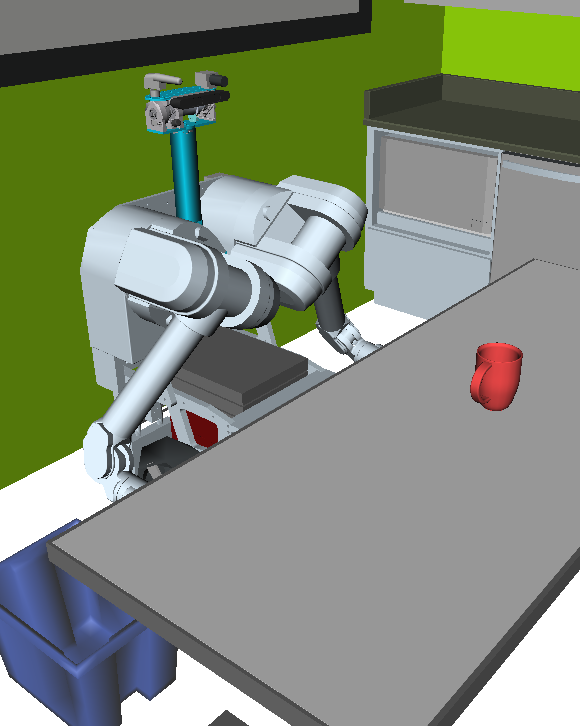
\includegraphics[width=0.185\linewidth]{figs/testherb-a.png}
   }
   \subfloat[Step 1, in $X_1$]{
      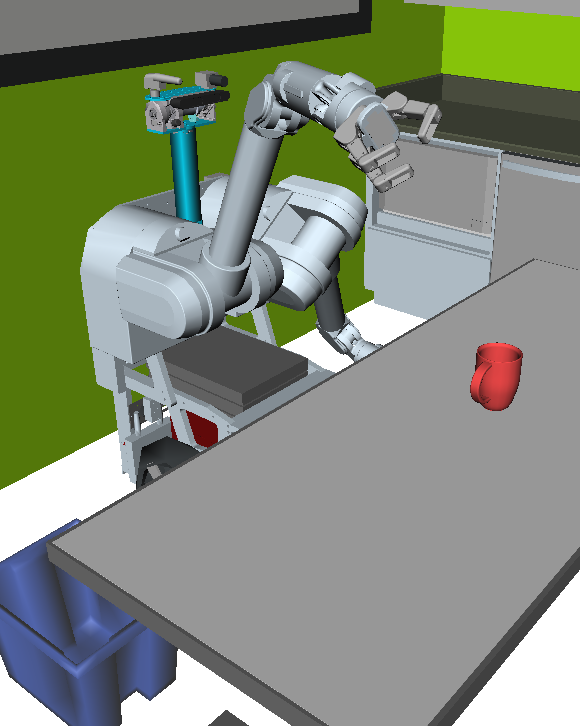
\includegraphics[width=0.185\linewidth]{figs/testherb-b.png}
   }
   \subfloat[Step 2, in $X_2$]{
      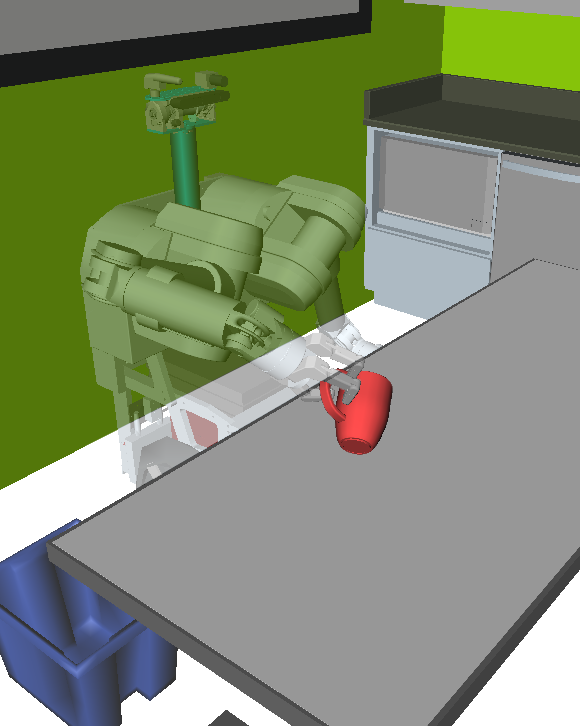
\includegraphics[width=0.185\linewidth]{figs/testherb-c.png}
   }
   \subfloat[Step 3, in $X_3$]{
      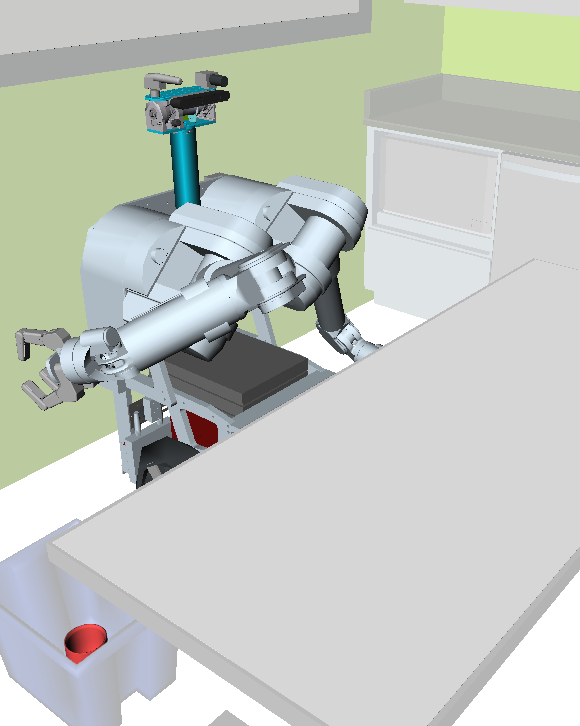
\includegraphics[width=0.185\linewidth]{figs/testherb-d.png}
   }
   \subfloat[Ending Configuration.]{
      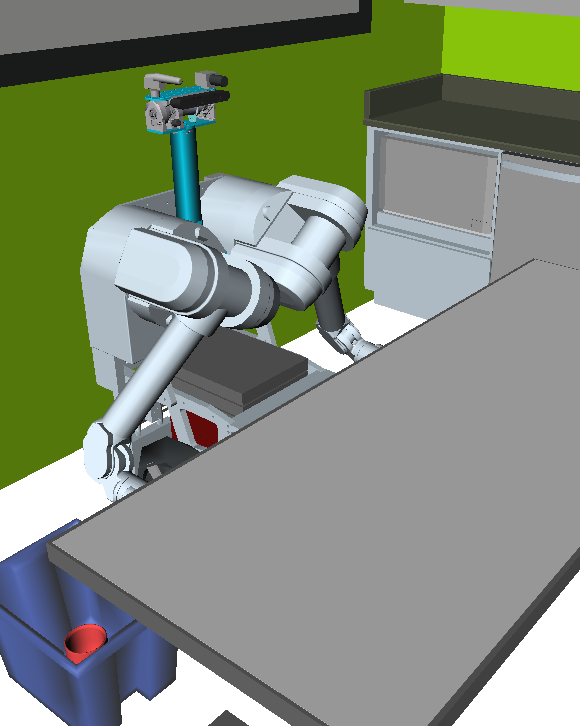
\includegraphics[width=0.185\linewidth]{figs/testherb-e.png}
   }

   \caption[][0.2in]{
     A home robot performing a three-step manipulation task.
     It must move from its home configuration
     to grasp the cup,
     transfer it to a drop location above the bin,
     and return home.
     Experimental results for the Multi-Set PRM
     are shown in Table~\ref{tab:testherb}}
   \label{fig:testherb-problem}
\end{figure*}

\begin{table*}
   \begin{widepage}
   \centering
   \footnotesize
   \setlength{\tabcolsep}{3pt}
   \renewcommand{\arraystretch}{1.3}
   \begin{tabular}{|cc|r@{ }lr@{ }lr@{ }lr@{ }l|r@{ }lr@{ }lr@{ }lr@{ }l|r@{ }lr@{ }lr@{ }lr@{ }l|}
   \toprule
   \multirow{2}{*}{Relations} & \multirow{2}{*}{Cost}
     & \multicolumn{8}{c|}{$\lambda = 0$}
     & \multicolumn{8}{c|}{$\lambda = 0.5$}
     & \multicolumn{8}{c|}{$\lambda = 1$}
   \\
     &
     & Step & 1 & Step & 2 & Step & 3 & \multicolumn{2}{c|}{Total}
     & Step & 1 & Step & 2 & Step & 3 & \multicolumn{2}{c|}{Total}
     & Step & 1 & Step & 2 & Step & 3 & \multicolumn{2}{c|}{Total}
   \\ \midrule
   \multirow{2}{*}{None} & Plan
     &  6.16&s &  3.72&s &  2.38&s & 12.25&s
     &  5.52&s &  2.89&s &  2.12&s & 10.53&s
     &  3.39&s &  2.25&s &  2.12&s &  7.76&s
   \\
     & Exec
     & 14.22&rad &  8.51&rad &  4.23&rad & 26.97&rad
     & 15.07&rad & 10.60&rad &  4.23&rad & 29.89&rad
     & 15.07&rad & 10.60&rad &  4.23&rad & 29.89&rad
   \\ [1ex]
   Inter-Step & Plan
     &  6.40&s &  2.33&s &  0.86&s &  9.59&s
     &  5.40&s &  1.55&s &  0.91&s &  7.86&s
     &  3.38&s &  0.91&s &  0.30&s &  4.59&s
   \\
   (Sec.~\ref{subsec:dynamic-environments},~\ref{subsec:grasped-objects})
     & Exec
     & 14.22&rad &  8.51&rad &  4.23&rad & 26.97&rad
     & 15.07&rad & 12.21&rad &  4.23&rad & 31.51&rad
     & 15.07&rad & 12.21&rad &  7.11&rad & 34.40&rad
   \\ [1ex]
   Self-Checked & Plan*
     &  3.54&s &  2.23&s &  1.17&s & 6.94&s
     &  2.99&s &  1.77&s &  1.16&s & 5.92&s
     &  1.47&s &  1.22&s &  1.16&s & 3.85&s
   \\
   (Sec.~\ref{subsec:cached-self-valid}) & Exec
     & 14.22&rad &  8.51&rad &  4.23&rad & 26.96&rad
     & 14.22&rad & 10.06&rad &  4.23&rad & 28.51&rad
     & 14.22&rad & 10.60&rad &  4.23&rad & 29.05&rad
   \\ [1ex]
   \multirow{2}{*}{Both} & Plan*
     &  3.25&s &  1.79&s &  0.90&s & 5.94&s
     &  2.88&s &  1.55&s &  0.92&s & 5.35&s
     &  1.47&s &  1.88&s &  0.31&s & 3.66&s
   \\
     & Exec
     & 14.22&rad &  8.51&rad &  4.23&rad & 26.96&rad
     & 14.22&rad &  8.51&rad &  4.23&rad & 26.96&rad
     & 14.22&rad &  9.64&rad &  6.36&rad & 30.22&rad
   \\ 
   \bottomrule
   \end{tabular}
   \caption[][0.2in]{Home robot manipulation task results.
     The entry with no relations and $\lambda=0$ is equivalent
     to the LazyPRM.}
   \label{tab:testherb}
   \end{widepage}
\end{table*}

We tested the Multi-Set PRM on the manipulation task
described in Fig.~\ref{fig:testherb-problem}.
We used the $r$-disk PRM construction rule with $r=2.0$ rad,
and a batch size of $N=1000$.
Planning times are measured on a Lenovo T430s laptop.
The planner was asked to solve each of the steps of the plan
sequentially.

We varied
(a) the planning vs. execution parameter $\lambda$
(see Section~\ref{subsec:alg-opt-path-cost}), and
(b) the subset relations provided to the planner
as described in Sections
\ref{subsec:dynamic-environments},
\ref{subsec:grasped-objects},
and \ref{subsec:cached-self-valid}.
We measured the time required for planning (s)
and the length of the resulting solution resulting path (rad)
for each step of the task.

Note that the Multi-Set PRM,
with no relations specified and $\lambda=0$
reduces to the Lazy PRM.
As expected,
increasing $\lambda$ resulted in decreased planning times
but yielded longer paths.
Including more $\mathcal{C}$-subset relations
also significantly reduced planning times,
and had little effect on path lengths on this problem.
Note that the planning time results when using
the cached self-collision-checked roadmap, denoted by (*),
do not include the pre-computation time.

Note that including inter-step relations drastically
reduces planning times for subsequent steps.
We expect this trend would continue as more steps are included.
Also, note that when $\lambda=0$,
path length is unchanged as the number of set relations is
changed
-- this is because the paths that are selected for evaluation
by the algorithm are a function only of their (constant) lengths.

%\subsection{Other Experiments to Run}
%
%\begin{itemize}
%\item with/without inter-step relations
%\item with/without padding
%\item with/without self-checked cache
%\item with/without relations for changing worlds
%\item with/without conservative boxes for grabbed objects
%\item constraints:
%   \begin{itemize}
%   \item handle with separate planner
%   \item handle with relaxed constraint, followed by local optimizer
%   \end{itemize}
%\item run optimizer on paths occasionally and/or before executing
%\end{itemize}


\subsection{Results and Behavior of the Multi-Set PRM}

See Figure~\ref{fig:broad-phase-2d}
for a simple example with integrated broad-phase collision checking
as described in Section~\ref{subsec:broad-phase}.

\begin{figure}
   \centering

   \subfloat[
      $\lambda=0$, no broad phase.
      Median planning cost: 6650
   ]{
      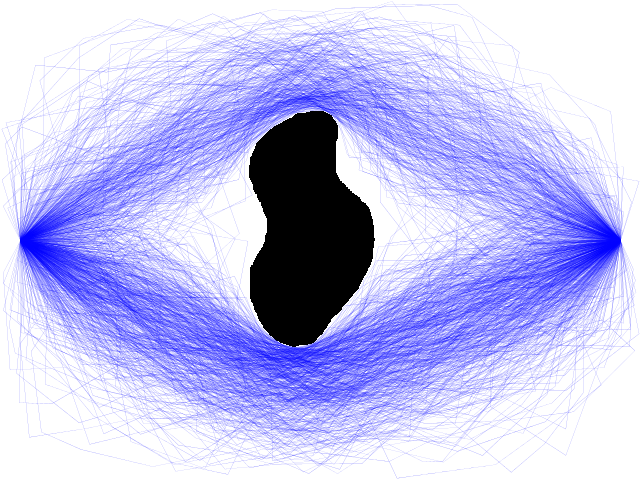
\includegraphics[width=0.45\linewidth]{figs/paths-lambda0-norel.png}
   }
   \subfloat[
      $\lambda=1$, no broad phase.
     Median planning cost: 4530
   ]{
      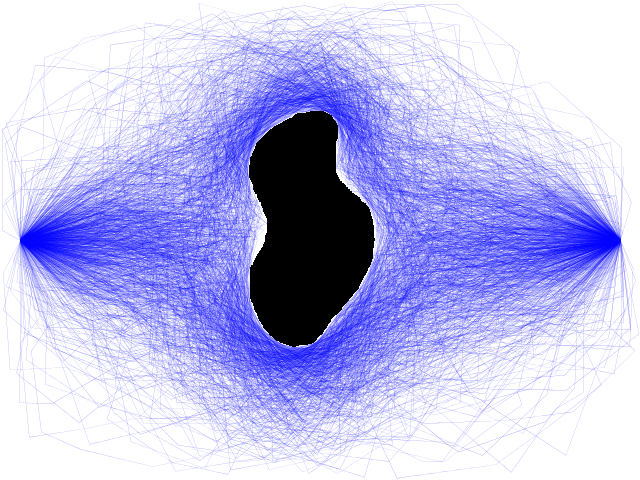
\includegraphics[width=0.45\linewidth]{figs/paths-lambda1-norel.png}
   }
   
   \subfloat[
      $\lambda=0$, with broad phase.
      Median planning cost: 2122
   ]{
      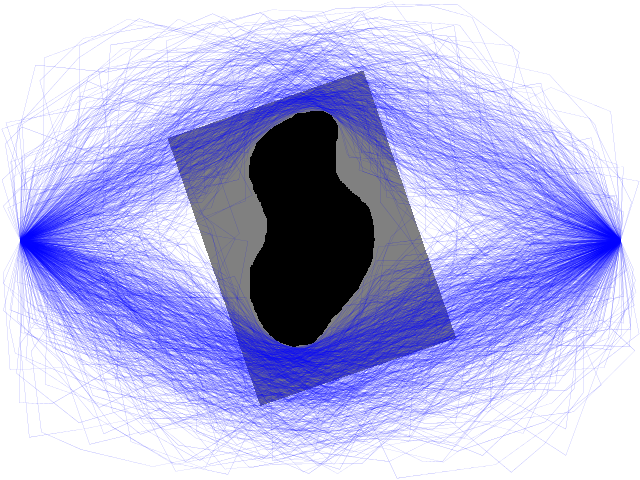
\includegraphics[width=0.45\linewidth]{figs/paths-lambda0-wrel.png}
   }
   \subfloat[
      $\lambda=1$, with broad phase.
      Median planning cost: 737
   ]{
      \includegraphics[width=0.45\linewidth]{figs/paths-lambda1-wrel.png}
   }

   \caption{A simple 2D example of the Multi-Set PRM using
     a broad-phase check.
     Checking for collision with the grey box is 10x less expensive
     than with the actual black obstacle.
     \cdnote{I need to talk about this in the text.}}
   \label{fig:broad-phase-2d}
\end{figure}


\section{Comprehensive Multi-Root Planning}
\label{chap:cmr}

While the Multi-Set PRM
allows planning computation to be reused between queries
across steps of a manipulation task,
a higher-level task planner must still distribute these queries
in order to discover a low-cost path
through all of the task's steps
(see Figure~\ref{fig:xx-diagram-multi-step}).
The types of queries we have discussed so far
(using sets
$V_{\mbox{\scriptsize start}}$ and $V_{\mbox{\scriptsize goal}}$)
take an \emph{any-to-any} form
-- the planner will return a successful path which connects
from any start to any goal vertex.
However,
when planning in parallel for multiple steps,
a task planner instead requires a \emph{diverse} set of
paths.

\begin{figure}
   \centering
   \subfloat[A real-world problem.]{
      \includegraphics[width=0.55\linewidth]{figs/herb-drilling.png}
      \label{subfig:herb-picture}
   }
   \caption{A real-world problem.}
   \subfloat[Illustration.]{
      \resizebox{0.35\linewidth}{!}{
      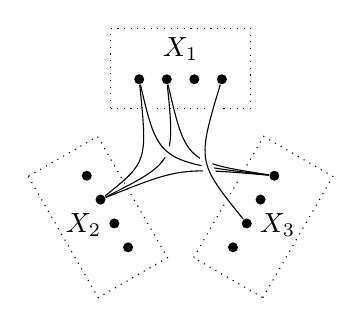
\begin{tikzpicture}[scale=0.7]

      \begin{scope}
      \node[rectangle,draw,dotted,
         inner sep=0,minimum height=0.4in,minimum width=0.7in] (x1) at (0,0) {};
      \node[below] at (x1.north) {$X_1$};
      \node[circle,inner sep=0,minimum size=0.05in,fill=black] (x1a) at (-0.75,-0.2) {};
      \node[circle,inner sep=0,minimum size=0.05in,fill=black] (x1b) at (-0.25,-0.2) {};
      \node[circle,inner sep=0,minimum size=0.05in,fill=black] (x1c) at ( 0.25,-0.2) {};
      \node[circle,inner sep=0,minimum size=0.05in,fill=black] (x1d) at ( 0.75,-0.2) {};
      \end{scope}

      \begin{scope}[shift={(-1.5,-2.7)},rotate=120]
      \node[rectangle,draw,dotted,rotate=120,
         inner sep=0,minimum height=0.4in,minimum width=0.7in] (x2) at (0,0) {};
      \node at (0,0.3) {$X_2$};
      \node[circle,inner sep=0,minimum size=0.05in,fill=black] (x2a) at (-0.75,-0.2) {};
      \node[circle,inner sep=0,minimum size=0.05in,fill=black] (x2b) at (-0.25,-0.2) {};
      \node[circle,inner sep=0,minimum size=0.05in,fill=black] (x2c) at ( 0.25,-0.2) {};
      \node[circle,inner sep=0,minimum size=0.05in,fill=black] (x2d) at ( 0.75,-0.2) {};
      \end{scope}

      \begin{scope}[shift={(1.5,-2.7)},rotate=-120]
      \node[rectangle,draw,dotted,rotate=-120,
         inner sep=0,minimum height=0.4in,minimum width=0.7in] (x3) at (0,0) {};
      \node at (0,0.3) {$X_3$};
      \node[circle,inner sep=0,minimum size=0.05in,fill=black] (x3a) at (-0.75,-0.2) {};
      \node[circle,inner sep=0,minimum size=0.05in,fill=black] (x3b) at (-0.25,-0.2) {};
      \node[circle,inner sep=0,minimum size=0.05in,fill=black] (x3c) at ( 0.25,-0.2) {};
      \node[circle,inner sep=0,minimum size=0.05in,fill=black] (x3d) at ( 0.75,-0.2) {};
      \end{scope}

      \draw (x1b) .. controls(-0.1,-1.7) .. (x2c);
      \draw[white,line width=4] (x1a) .. controls(-0.4,-1.7) .. (x3a);
      \draw (x1a) .. controls(-0.4,-1.7) .. (x3a);
      \draw (x1b) .. controls( 0.1,-1.7) .. (x3a);
      \draw (x1a) .. controls(-0.6,-1.7) .. (x2c);
      \draw (x3a) .. controls(0.0,-1.8) .. (x2c);
      \draw[white,line width=4] (x1d) .. controls( 0.3,-1.7) .. (x3c);
      \draw (x1d) .. controls( 0.3,-1.7) .. (x3c);

      \end{tikzpicture}
      }
      \label{subfig:cmr-illustration}
   }
   \caption{The comprehensive multi-root (CMR) problem.}
   \label{fig:cmr-problems}
\end{figure}

To handle this,
we formulate and study the
\emph{comprehensive multi-root} (CMR) planning problem
\cite{dellin2015cmr} (Figure~\ref{fig:cmr-problems}),
in which feasible paths are desired between multiple regions.
We propose two primary contributions which allow us to extend
state-of-the-art sampling-based planners.
First, we propose the notion of \emph{vertex coloring} as a compact
representation of the CMR objective on graphs.
Second, we propose a method for \emph{deferring edge evaluations}
which do not advance our objective, by way of a simple
criterion over these vertex colorings.
The resulting approach can be applied to any CMR-agnostic 
graph-based planner which evaluates a sequence of edges.
We prove that the theoretical performance of the colored algorithm
is always strictly better than (or equal to)
that of the corresponding uncolored version.
We then apply the approach to the Probabalistic RoadMap (PRM)
algorithm;
the resulting \emph{Colored Probabalistic RoadMap} (cPRM)
is illustrated on 2D and 7D CMR problems.

\subsection{The Comprehensive Multi-Root Problem}

We work with the robot's configuration space $\mathcal{C}$
and its collision-free subset $\mathcal{C}_{\mbox{\scriptsize free}}$.
We consider the general problem with $N$ root sets in this space
$\{ X_1, \dots, X_N \}$.
We seek a diverse set of feasible paths between root sets
-- that is, we want to maximize the number of connected roots between sets. 
We call this the \emph{comprehensive multi-root} (CMR) planning problem.

We track progress via the $r$-score:
\begin{equation}
   r = \big| \{
      \textsc{Path}(x_a,x_b) \;|\; x_a,x_b~\text{in different root sets}
      \} \big|.
   \label{eqn:obj}
\end{equation}
For example, the solution illustrated in Figure~\ref{subfig:cmr-illustration}
has an $r$-score of 6 out of a maximum of 27.
Our objective is to \emph{maximize} the $r$-score as \emph{quickly} as
possible.

\subsection{A CMR Example}

\begin{figure*}[t]
   %\begin{widepage}
   \centering
   \begin{minipage}{.55\textwidth}
      \subfloat[PRM (86 Edges Checked) (195 Edges Considered, No Pairs)]{
         \includegraphics{build/w13-fu1-ec86}
         \label{subfig:w13-sameec-uncolored}
      }
      \subfloat[cPRM (86 Edges Checked) (344 Edges Considered, 1 Pair)]{
         \includegraphics{build/w13-fs1-ec86}
      }
      \\ \quad \\
      \subfloat[PRM (344 Edges Considered) (125 Edges Checked, 8 Pairs)]{
         \includegraphics{build/w13-fu1-ei344}
         \label{subfig:w13-sameein-uncolored}
      }
      \subfloat[cPRM (344 Edges Considered) (91 Edges Checked, 8 Pairs)]{
         \includegraphics{build/w13-fs1-ei344}
         \label{subfig:w13-sameein-colored}
      }
   \end{minipage}
   \begin{minipage}{.43\textwidth}
      \subfloat[Edges considered, evaluated, deferred, and skipped.]{
         \includegraphics{build/plot-edges-w13}
         \label{subfig:w13-plot-edges}
      }
      \\ \quad \\
      \subfloat[CMR Objective vs edges evaluted.]{
         \begin{tikzpicture}[font=\scriptsize]
         % primary axis
         \begin{axis}[
            xlabel={Edges Checked},
            ylabel={Pairs Connected},
            %legend pos= north west,
            legend style={at={(axis cs:5,7.5)},anchor=north west},
            legend cell align=left,
            %axis equal image,
            width=3.4in,
            height=1.3in,
            xmin=0, xmax=150,
            %xmin=0, xmax=1000, ymin=0,
            %scaled ticks=base 10:-3,
            xlabel near ticks,
            ylabel near ticks]
         \addplot[black,ultra thick] table[col sep=space] {figs/w13-fu1-qs-pvc.txt};
         \addlegendentry{Uncolored}
         \addplot[mark=*,black,only marks,mark size=1,forget plot] plot coordinates {
            (125,8) % uc
         };
         \addplot[green,thick] table[col sep=space] {figs/w13-fs1-qs-pvc.txt};
         \addlegendentry{Colored}
         \addplot[mark=*,black,only marks,mark size=1,forget plot] plot coordinates {
            (86,1) %+1
            (87,2) %+1
            (89,4) %+2
            (90,6) %+2
            (91,8) %+2
         };
         \addplot[blue,mark=o,mark size=2] plot coordinates {(86,0) (86,1)}; % a-b comparison
         \addplot[blue,mark=o,mark size=2] plot coordinates {(125,8) (91,8)}; % c-d comparison
         % coordinates
         \coordinate (subfig_a_point) at (axis cs: 86,0);
         \coordinate (subfig_b_point) at (axis cs: 86,1);
         \coordinate (subfig_c_point) at (axis cs: 125,8);
         \coordinate (subfig_d_point) at (axis cs: 91,8);
         \end{axis}
         % labels
         \node[circle,inner sep=0pt,color=blue,fill=white] (subfig_b_label) at (2.9,0.6) {(b)};
         \node[circle,inner sep=0pt,color=blue,fill=white] (subfig_d_label) at (3.1,1.3) {(d)};
         \node[circle,inner sep=0pt,color=blue,fill=white] (subfig_a_label) at (4.9,0.5) {(a)};
         \node[circle,inner sep=0pt,color=blue,fill=white] (subfig_c_label) at (5.2,1.2) {(c)};
         \draw[color=blue,->] (subfig_b_label) -- ($ (subfig_b_point)!4pt!(subfig_b_label) $);
         \draw[color=blue,->] (subfig_d_label) -- ($ (subfig_d_point)!4pt!(subfig_d_label) $);
         \draw[color=blue,->] (subfig_a_label) -- ($ (subfig_a_point)!4pt!(subfig_a_label) $);
         \draw[color=blue,->] (subfig_c_label) -- ($ (subfig_c_point)!4pt!(subfig_c_label) $);
         \end{tikzpicture}
         \label{subfig:w13-plot-pairs}
      }
   \end{minipage}
   \caption[][0.2in]{A comparison between an
      uncolored~(\ref{subfig:w13-sameec-uncolored},\ref{subfig:w13-sameein-uncolored})
      and colored~(\ref{subfig:w13-sameec-colored},\ref{subfig:w13-sameein-colored})
      forest-of-trees PRM on the same sequence of edges.
      Plot~(\ref{subfig:w13-plot-edges}) shows the evolution of edges in both
      algorithms as they progress,
      and plot~(\ref{subfig:w13-plot-pairs}) shows the number of between-rootset
      pairs found by each.}
   \label{fig:example-w13-figstar}
   %\end{widepage}
\end{figure*}

See Figure~\ref{fig:example-w13-figstar}
for a sample CMR problem between a set of start vertices (at top)
and a set of goal vertices (at bottom).
This example uses a simple forest-of-trees PRM construction rule.

\section{Task Planning}
\label{chap:task-planning}

\subsection{The \textsc{Proteus} Task Planner}

I propose to write a simple task planner,
\textsc{Proteus}
(\textsc{Proteus} Reasons Over Task Effort Using Sampling).
For a specified coupled manipulation planning problems,
it will compute its multi-set structure
and call into parallel instances of the Multi-Set PRM for each step
using the CMR objective
in order to find a solution path.
This will allow for full-scope experimental evaluations to be conducted
on the approach.
We assume the step decomposition is provided by either
a human operator or symbolic planner.

\textbf{Related Work.}
\cdnote{There is a large body of related work in the area of subgoal planning
that is relevant to the design of this task planner that I
should reference here.}

\textbf{Interleaved Planning and Execution.}
While primary comparisons
will consider planning in a separate phase from execution,
\textsc{Proteus} will also support a simple version of
interleaved planning execution
for comparison to baseline approaches which commit to early choices.
In fact, the approach in this thesis is
amenable to interleaved planning and execution,
since the Multi-Set PRM can continually updated
the $q_{\mbox{\scriptsize init}}$ configuration.
See research question \ref{ques:proteus-compare} for details.
